\documentclass[a4paper,11pt,twoside,ngerman,color]{book}

% header.tex
\usepackage[a4paper,left=3.5cm,right=2.5cm,bottom=3.5cm,top=3cm]{geometry}

\usepackage[pdftex]{graphicx,color}
\usepackage{amsmath,amssymb,subfigure}
\usepackage{rotating}

% Theorem-Umgebungen
\usepackage[amsmath,thmmarks]{ntheorem}

% Korrekte Darstellung der Umlaute
\usepackage[utf8]{inputenc}
\usepackage[T1]{fontenc}
\usepackage{german}

% Algorithmen
\usepackage[ruled,vlined]{algorithm2e}
\usepackage{algorithmic}

\usepackage{enumerate}
\usepackage{listings}
\usepackage{hyperref}


% Bibtex deutsch
\usepackage{bibgerm}

% URLs
\usepackage{url}

% Caption Packet
\usepackage[margin=0pt,font=small,labelfont=bf]{caption}
% Gliederung einstellen
%\setcounter{secnumdepth}{5}
%\setcounter{tocdepth}{5}

% Theorem-Optionen %
\theoremseparator{.}
\theoremstyle{change}
\newtheorem{theorem}{Theorem}[section]
\newtheorem{satz}[theorem]{Satz}
\newtheorem{lemma}[theorem]{Lemma}
\newtheorem{korollar}[theorem]{Korollar}
\newtheorem{proposition}[theorem]{Proposition}
% Ohne Numerierung
\theoremstyle{nonumberplain}
\renewtheorem{theorem*}{Theorem}
\renewtheorem{satz*}{Satz}
\renewtheorem{lemma*}{Lemma}
\renewtheorem{korollar*}{Korollar}
\renewtheorem{proposition*}{Proposition}
% Definitionen mit \upshape
\theorembodyfont{\upshape}
\theoremstyle{change}
\newtheorem{definition}[theorem]{Definition}
\theoremstyle{nonumberplain}
\renewtheorem{definition*}{Definition}
% Kursive Schrift
\theoremheaderfont{\itshape}
\newtheorem{notation}{Notation}
\newtheorem{konvention}{Konvention}
\newtheorem{bezeichnung}{Bezeichnung}
\theoremsymbol{\ensuremath{\Box}}
\newtheorem{beweis}{Beweis}
\theoremsymbol{}
\theoremstyle{change}
\theoremheaderfont{\bfseries}
\newtheorem{bemerkung}[theorem]{Bemerkung}
\newtheorem{beobachtung}[theorem]{Beobachtung}
\newtheorem{beispiel}[theorem]{Beispiel}
\newtheorem{problem}{Problem}
\theoremstyle{nonumberplain}
\renewtheorem{bemerkung*}{Bemerkung}
\renewtheorem{beispiel*}{Beispiel}
\renewtheorem{problem*}{Problem}

% Algorithmen anpassen %
\renewcommand{\algorithmicrequire}{\textit{Eingabe:}}
\renewcommand{\algorithmicensure}{\textit{Ausgabe:}}
% \floatname{algorithm}{Algorithmus}
% \renewcommand{\listalgorithmname}{Algorithmenverzeichnis}
% \renewcommand{\algorithmiccomment}[1]{\color{grau}{// #1}}

% Zeilenabstand einstellen %
\renewcommand{\baselinestretch}{1.25}
% Floating-Umgebungen anpassen %
\renewcommand{\topfraction}{0.9}
\renewcommand{\bottomfraction}{0.8}
% Abkuerzungen richtig formatieren %
\usepackage{xspace}
\newcommand{\vgl}{vgl.\@\xspace} 
\newcommand{\zB}{z.\nolinebreak[4]\hspace{0.125em}\nolinebreak[4]B.\@\xspace}
\newcommand{\bzw}{bzw.\@\xspace}
\newcommand{\dahe}{d.\nolinebreak[4]\hspace{0.125em}h.\nolinebreak[4]\@\xspace}
\newcommand{\etc}{etc.\@\xspace}
\newcommand{\evtl}{evtl.\@\xspace}
\newcommand{\ggf}{ggf.\@\xspace}
\newcommand{\bzgl}{bzgl.\@\xspace}
\newcommand{\so}{s.\nolinebreak[4]\hspace{0.125em}\nolinebreak[4]o.\@\xspace}
\newcommand{\iA}{i.\nolinebreak[4]\hspace{0.125em}\nolinebreak[4]A.\@\xspace}
\newcommand{\sa}{s.\nolinebreak[4]\hspace{0.125em}\nolinebreak[4]a.\@\xspace}
\newcommand{\su}{s.\nolinebreak[4]\hspace{0.125em}\nolinebreak[4]u.\@\xspace}
\newcommand{\ua}{u.\nolinebreak[4]\hspace{0.125em}\nolinebreak[4]a.\@\xspace}
\newcommand{\og}{o.\nolinebreak[4]\hspace{0.125em}\nolinebreak[4]g.\@\xspace}
\newcommand{\oBdA}{o.\nolinebreak[4]\hspace{0.125em}\nolinebreak[4]B.\nolinebreak[4]\hspace{0.125em}d.\nolinebreak[4]\hspace{0.125em}A.\@\xspace}
\newcommand{\OBdA}{O.\nolinebreak[4]\hspace{0.125em}\nolinebreak[4]B.\nolinebreak[4]\hspace{0.125em}d.\nolinebreak[4]\hspace{0.125em}A.\@\xspace}

% Leere Seite ohne Seitennummer, naechste Seite rechts
\newcommand{\blankpage}{
 \clearpage{\pagestyle{empty}\cleardoublepage}
}

% Keine einzelnen Zeilen beim Anfang eines Abschnitts (Schusterjungen)
\clubpenalty = 10000
% Keine einzelnen Zeilen am Ende eines Abschnitts (Hurenkinder)
\widowpenalty = 10000 \displaywidowpenalty = 10000
% EOF


\begin{document}
% Titelseite
\begin{titlepage}
\vspace*{-2cm}
\newlength{\links}
\setlength{\links}{-1.5cm}
\sf
\LARGE

\hspace*{\links}
\begin{minipage}{12.5cm}

\includegraphics[width=8cm]{bilder/tulogo-rgb}
%\hspace*{-0.25cm} \textbf{TECHNISCHE UNIVERSITÄT DORTMUND}\\
%\hspace*{-1.2cm} \rule{5mm}{5mm} \hspace*{0.1cm} FACHBEREICH INFORMATIK\\
\end{minipage}

\vspace*{4cm}

\hspace*{\links}
\hspace*{-0.2cm}
\begin{minipage}{9cm}
\large
\begin{center}
{\Large Masterarbeit} \\
\vspace*{1cm}
\bf{ Vollautomatischer explorativer Crawler-Test von grafischen Oberflächen } \\
\vspace*{1cm}
Matthäus Poloczek\\
\today
\end{center}
\end{minipage}

\vspace*{5.5cm}

\hspace*{\links}

\vspace*{1.5cm}

\vspace*{.6cm}

\hspace*{\links}
\begin{minipage}[b]{5cm}
\normalsize
\raggedright
Betreuer: \\
Prof. Dr. Rudolph \\
Dr. Windmüller, e-Spirit AG \\
\end{minipage}

\definecolor{TUGreen}{rgb}{0.517,0.721,0.094}
\vspace*{2.5cm}
\hspace*{\links}
\begin{minipage}[b]{8cm}
\normalsize
\raggedright
Fakultät für Informatik\\
Algorithm Engineering (Ls11)\\
Technische Universität Dortmund \\
http://ls11-www.cs.tu-dortmund.de
\end{minipage}


\end{titlepage}

\blankpage
%\include{chapters/titelseite_innen}
%\blankpage

\pagenumbering{roman}
\tableofcontents
\cleardoublepage
\pagenumbering{arabic}

% Kapitel
\iffalse
% das iffalse verhindert, dass irgendetwas bis zum \fi von latex verarbeitet wird.
% beginn latex-cheatsheet

%Neue seite:
\newpage

%Zitat:
\cite{website:biu}

%Kapitelnummer:
\ref{problems}

%Seitennummer:
\pageref{fig:mvcpattern}

%Hyperlink:
\url{http://www.freesound.org/}

%Anfuehrungszeichen:
\glqq{}Derp\grqq{}

% Bild:
\begin{figure}
	\centering
	\includegraphics[width=0.75\textwidth]{bilder/mammenkonzept2.jpg}
	\caption{Längerer Beschreibungstext Lorem Ipsum etc}
	\label{fig:application_lifecycle_diagram}
\end{figure}

%Bildverweis:
\ref{fig:application_lifecycle_diagram}

% Liste:
\begin{itemize}
  \item \textsc{Tap} heisst Tippen oder Klicken
  \item \textsc{Pan} ist eine Berührung des Spielfelds
  \item \textsc{Pinch} bedeutet die Berührung oder Ziehen von zwei Punkten oder Pans gleichzeitig.
  \item \textsc{Zoom} bedeutet Pinch mit Veränderung der Distanz zwischen den Berührpunkten.
\end{itemize}

% Algorithmus:
\begin{algorithm} \SetAlgoLined \KwData{Vektormenge $A$; Koordinaten $x,y$; maximale vorkommende Vektorlänge $max$} \KwResult{$A$ enthält neues Optimum und Zwischenwerte } $x,y$ in Weltkoordinaten bringen\; $vx \in A \longleftarrow x,y$ auf den nächsten Wert interpoliert\; \For{Vektor $v \in A$}
  {
   \If{$v.length \geq vx.length$}
	  {
	   $v.coords \longleftarrow vx.coords$\;
	  }
		$max \longleftarrow max(max, v.length)$\;
	 } \caption{Update Fuzzy Map mit neuem Vektor} \label{alg:swarmalgo}
\end{algorithm}

% ende latex-cheatsheet
\fi



% einleitung.tex
\chapter{Einleitung}\label{intro}


Ein Hauptproblem der Softwareentwicklung ist der langwierige, häufig nichtdeterministische
Prozess des Testens bzw. der Qualitätssicherung und die damit verbundenen hohen Kosten.
Dies gilt insbesonders, wenn die Entwickler selbst beteiligt sind.
Bekannte Ansätze zur Lösung dieses Problems sind z.B. die Durchführung von Tests
durch dedizierte (weniger kostspielige) Tester, oder auch die Automatisierung von Tests. 
 
Speziell für den Fall von in der Industrie weit verbreiteten graphischen Nutzeroberflächen
mittels \textbf{Java Swing} \cite{JavaSwing} gibt es zahlreiche Möglichkeiten variierender
Komplexität wie z.B. \textbf{QF-Test} \footnote{\url{ http://www.qfs.de/en/qftest/index.html }},
\textbf{uispec4j} \footnote{\url{ https://github.com/UISpec4J/UISpec4J }},
\textbf{FEST} \footnote{\url{ https://code.google.com/p/fest/ }} oder auch 
\textbf{Jemmy} \footnote{\url{ https://jemmy.java.net/ }}. Viele bieten selbst interaktive
GUIs zur nutzerfreundlichen Testerstellung, erweiterbare Module und die Möglichkeit eigener Skripte. Auch
Integration von \textbf{JUnit} \footnote{\url{ http://junit.org/ }} oder 
\textbf{TestNG} \footnote{\url{ http://testng.org/doc/index.html }}
und Eclipse-Unterstützung \footnote{\url{ http://www.eclipse.org/ }} sind verbreitet. Was diese
Lösungsmöglichkeiten allerdings gemeinsam haben, ist die notwendige VORGABE der
durchzuführenden Eingaben und der erwarteten, zu überprüfenden Resultate. Dies ist
insofern ein Problem, dass ein Entwickler, der eine bestimmte, evtl. abwegige Eingabe nicht
voraussieht, vermutlich auch keinen Test dafür vorsehen wird. Selbst ein Tester wird unter
Umständen nicht ALLE, insbesondere auch die ungültigen, möglichen Eingabekombinationen probieren.
Dann gibt es noch weitere, schwer mit einer europäischen Tastatur zu erstellende, oder auch unsinnige Varianten. 
 


\section{Ziel dieser Arbeit}\label{structurelatex}


Der hier vorgestellte Vorschlag wird nun in einem neuen Werkzeug resultieren, welches vollautomatisch
funktioniert und das
sich nicht primär mit dem gewünschten und erwartetem Verhalten der getesteten GUI beschäftigt, sondern
vielmehr systematisch Vertreter aller technisch möglichen Eingaben (Sonderzeichen, extrem
lange Eingaben etc.) eingibt. Es wird völlig selbsttätig Knöpfe und Eingabemasken einer zu testenden
Applikation erkennen, systematisch mögliche Eingabe-Kombinationen durchprobieren, und für eventuelle
Folgebildschirme oder sich auf Knopfdruck öffnende neue Bildschirmelemente dasselbe tun.
Wenn eine sinnhaltiger Anmeldung o.Ä. nötig ist, um an die
\glqq{}Interna\grqq{} eines Programms zu kommen, muss das natürlich dennoch manuell vorgesehen oder
durchgeführt werden. Ebenso sollten Eingaben eines gewissen Kontexts (z.B. \glqq{}Programm beenden\grqq{})
vermieden werden, welche den Test vorzeitig beenden könnten.
 
Das Vorgehen des Werkzeugs soll dann in einer Baum- oder Graphartigen
Struktur mitprotokolliert werden - hierfür wird \textbf{JGraphT} verwendet \footnote{\url{ http://http://jgrapht.org/ }} --
um einerseits auch bei sich selbsttätig oder durch Eingaben schließenden Elementen diese wieder
neu zu öffnen, um alle Eingaben ausprobieren zu können, oder auch, um auftretende Zyklen 
zu erkennen sowie um erzeugte und erkannte Fehler letztendlich zu reproduzieren.
Eine ansehnliche Visualisierung btw. Modellierung des getesteten Programms, die
im Anschluss durch jedwedes kompatibles Graph-Visualisierungs-Programm
durchgeführt werden kann, ist ein angenehmer Seiteneffekt.

Es ist unrealistisch, z.B. in
einem Texteingabefeld jeden existierenden String zu probieren, hier muss eine möglichst
fehlertreibende und dennoch endliche Untermenge gefunden werden.

Schaltbare Elemente oder Auswahlen stellen ebenso
eine potenziell unüberschaubare Zustandsmenge der Applikation dar und müssen für eine
zufriedenstellende Abdeckung möglicher Anwendungsfälle mithilfe von
Pseudozufallsmethoden getestet werden. Überlegungen bezüglich eventuell überdauernder Programmeinstellungen
aus vorherigen Tests sind auch nötig -- zufällige Tastendrücke könnten zu irreversiblen Schäden an
Programmdateninhalten führen, und weitere Tests einschränken oder irrelevant machen. Ein Rücksetzen
der Applikation auf einen ursprünglichen Gesamtzustand ist also evtl. notwendig, soweit anwendbar.
 
Weiterhin gibt verschiedene Ansätze, so einen Test durchzuführen: Sollte überhaupt die
grafische Oberfläche erzeugt und dann Mausklicks darauf simuliert werden? Oder sollte der
Tester eher alle möglichen Kontrollflüsse quasi statisch bzw. offline ausführen? Resultierende
Fehler und Meldungen sollten geeignet von den System- und Errorstreams gelesen und
protokolliert werden, und man könnte auch eine Schnittstelle für auftretende Exceptions oder
Runtime-Errors vorsehen oder sie aus der Applikation abfangen oder mitschneiden. 
 
Die Entwicklung und Implementierung sowie die Anwendung dieses Werkzeugs auf eine Java-Swing-Applikation
der \textbf{e-Spirit AG}, \textbf{FirstSpirit} 
\footnote{\url{ http://www.e-spirit.com/de/produkt/arbeiten-mit-firstspirit/usability-fuer-redakteure/ }}, 
ist der geplante 
Umfang dieser Abschlussarbeit. Zunächst werden existierende Methoden und Lösungen der automatisierten
Testverfahren auf graphischen Oberflächen betrachtet und im Kontext zum hier vorgestellten Konzept
bewertet.

Einige sich anbietende Erweiterungen dieses Prinzips wären die Unterstützung anderer graphischen Bibliotheken
der Java-Infrastruktur. Als Beispiele genannt seien SWT, das u.A. von eclipse genutzt wird,
oder auch die speziellen Bibliotheken, die für Android-Applikationen genutzt werden.
Diese sind swing sehr ähnlich, basieren aber auf einem xml-Format zur Definition der
Oberflächenstruktur, um eine Entkopplung der Darstellung von der Funktionalität zu erreichen.
Unglücklicherweise würde dies vermutlich dazu führen, dass verschiedene Versionen des
Android-Betriebssystems unterschiedliche Implementationen seitens eines vollautomatischen
Testers nötig machen.
 
Weitere Überlegungen, die vermutlich nicht mehr im Umfang dieser Master-Arbeit sein
würden, aber die z.B. als Erweiterungsmöglichkeiten genannt werden könnten, sind die
Nutzung von Bilderkennung / Computer Vision, um auch über Java hinaus GUIs testen zu
können. Hierbei muss natürlich die Beschriftung von Knöpfen wiedererkannt werden können,
und viele GUIs benutzen Glyphen anstelle beschrifteter Schaltflächen. 

%%% TeX-master: "../main.tex"
% kapitel2.tex
\chapter{Funktionstests graphischer Oberflächen}\label{chapter:introguitesting}


Dieses Kapitel befasst sich mit einigen in der Industrie verbreiteten bzw. \glqq{}State of the Art\grqq{}-Lösungen
für das Problem automatischer GUI-Tests, dazu mit in einem Artikel sowie einer Doktorarbeit
vorgestellten Methoden. 
Es werden verschiedene Lösungen (für Java-Swing und andere) vorgestellt,
ihr jeweiliger Implementationsaufwand begutachtet sowie eventuelle Vor- und Nachteile aufgezeigt.
Auch wenn bereits im Ansatz ein Unterschied zum hier vorgestellten Konzept besteht, kann man dennoch
Aufwand und Nutzen sowie Vor- und Nachteile vergleichen.


\section{Grundlagen: Unterschiede Testverfahren}\label{section:testingapproaches}


\section{Automatisierte GUI-Tests}\label{section:automatedguitesting}


\textbf{uispec4j} \footnote{\url{ https://github.com/UISpec4J/UISpec4J }} ist ein Java-Programm 
zum Test von graphischen Nutzeroberflächen
in Java. Es wird ein Programm implementiert, welches parallel zur zu testenden GUI läuft,
vorgegebene Eingaben vornimmt und im Anschluss einen gewünschten Zustand in den Elementen der GUI
überprüfen kann. Ein Problem ist dabei, dass nur oberflächliche Dinge geprüft werden können,
wie z.B. die Existenz oder das Fehlen eines fest definierten Fensters oder Elements. Andererseits muss für jede
Prüfanfrage ein Entwickler ein entsprechendes Testsegment schreiben. Die Applikation muss also
zumindest doppelt implementiert werden, was in einem hohen Aufwand resultiert.

\vspace{0.5cm}

\textbf{fest} \footnote{\url{ https://code.google.com/p/fest/ }} oder 
\glqq{}Fixtures for Easy Software Testing\grqq{} verfolgt denselben Ansatz.
Es agiert als Kontrollprogramm auf einer zu testenden Applikation und kann gewisse Prüfungen
auf dieser ausführen. Tatsächlich sind die beiden praktisch identisch, bauen sie doch beide
auf JUnit \footnote{\url{ http://junit.org/ }} auf und erweitern dieses.

\vspace{0.5cm}

\textbf{QF-Test} \footnote{\url{ http://www.qfs.de/en/qftest/index.html }} 
bietet darüber hinaus eine eigene graphische Nutzeroberfläche
und ein sogenanntes \glqq{}Capture / Replay\grqq{}-System. Hierbei soll es Entwicklern erspart bleiben,
Tests als Programme zu implementieren, stattdessen bedient ein Tester durch die QF-Test-Maske
hindurch ein zu prüfendes Programm, während die Eingaben und Ausgaben mitgeschnitten werden.
Diese Aufnahme des Programmverhaltens gilt dann als \glqq{}Sollverhalten\grqq{} und wird in Folge
durch automatisierte Wiederholung verglichen und geprüft. Dieselbe Serie von Eingaben muss
bei Testdurchläufen eine identische Ausgabe zu diesem Soll hervorrufen, ansonsten
wird ein Fehler im Programm vermutet. Dieser Fehler kann auch eine gewünschte Programmveränderung sein.

Da allerdings hier ein Tester und nicht ein Entwickler die Tests erstellt und pflegt, ist dieses
Verfahren arbeitszeittechnisch wesentlich effizienter als vorherige Methoden. Ein Tester muss
nicht die Innereien des Programms verstehen oder verstehen können. Er muss das Programm lediglich
bedienen können. Ebenso sind keine Programmierkenntnisse notwendig.


\subsection{Kontinuierliche Qualitätskontrolle von Webanwendungen auf Basis 
maschinengelernter Modelle}\label{ssection:windmueller}


Die \glqq{}Dissertation Kontinuierliche Qualitätskontrolle von Webanwendungen auf 
Basis maschinengelernter Modelle\grqq{} \cite{diss:windmueller} stellt ein neuartiges Konzept
zur Überprüfung des Verhaltens einer Applikation vor. Die Idee ist, mithilfe eines
lernenden Algorithmus nach Angluin \cite{angluin} einen Automaten bzw. ein komplettes Modell
der dem Algorithmus unbekannten, quasi \glqq{}Black Box\grqq{}, Anwendung zu erstellen und zu vergleichen.

Hierzu muss aber erwähnt werden, dass lediglich der das Modell erstellende Algorithmus nicht
weiss, was das Programm macht - seitens des Testers ist erheblicher Aufwand für die Implementation
von sogenannten Treibern notwendig, die jede mögliche Eingabe an die Anwendung bzw. jedes
mögliche Wort des Eingabealphabets abdeckt. Ebenso müssen die bei Webanwendungen normierten
Antworten auf die Eingaben gelesen und für Zustandsabbildung genutzt werden. Diese Treiber
sind hochspezifisch für eine Anwendung und müssen sogar für verschiedene Versionen derselben
Anwendung neu angepasst werden.

Zurück zum Prinzip: Als Resultat existieren nun die erlernten Modelle der Anwendung bzw. spezifischer
Versionen der Anwendung. Diese kann man nun mit einem Algorithmus vergleichen und Unterschiede
herausstellen. Solche entstehen letztendlich nur aus zwei Gründen: Die Anwendung wurde verändert
und es tritt eine gewünschte Funktionsänderung oder -erweiterung auf, oder ein neuartiger Fehler
wurde (im Vergleich zur letzten Version) erschaffen. Diese Differenz ist offensichtlich nur
aus dem Kontext heraus und nur durch einen Menschen zu verstehen.

Insofern handelt es sich um eine Form des Regressionstests \cite{regression} - bestehende bzw.
vorherige Funktion wird mit einem Momentanzustand verglichen und Diskrepanzen aufgedeckt. Der
Ansatz hat dementsprechend dieselben Nachteile - jede gewünschte Änderung des Systems muss eine
Neueinstellung oder Neuerstellung der Testkonfiguration nach sich ziehen. Bei häufigen
Änderungen kann der Aufwand der Testerstellung schnell dem Entwicklungsaufwand gleichkommen bzw.
diesen sogar überschreiten.

Der Vorteil ist natürlich genauso, dass selbst geringfügige Abweichungen im Verhalten sofort
auffallen und zur Analyse markiert werden. So wurden beim Praxiseinsatz auf verschiedenen
Webanwendungen und ihren Versionskontrollsystemen bis dato unerkannte Programmfehler entdeckt.
Diese wurden durch Eigenarten und Konzepte der bestehenden Tests maskiert und unsichtbar.
Eine offensichtliche Schlussfolgerung ist, dass mehr und verschiedene Tests zu besseren
Ergebnissen führen - das Problem liegt, wie immer, im Aufwand.

Verglichen mit einem gewöhnlichen Regressionstest erspart dieser Ansatz dem Nutzer
bzw. Entwickler die Definition der Zustandsfolgen. Zu beachten ist allerdings wieder:
Es gibt für den Algorithmus kein richtig oder falsch, nur Unterschiede zwischen Versionen.
Ein normaler GUI-Test definiert üblicherweise eine erwartete Antwort oder Reaktion auf einen
bestimmten Knopfdruck. Hier würde so lange kein \glqq{}Problem\grqq{} auftreten, wie das Verhalten eines
Programms konsistent ist, selbst wenn dieses Verhalten an sich eigentlich fehlerhaft ist.

Es gibt noch ein weiteres für das hier vorgestellte Konzept interessantes Feature,
den sogenannten reuse-Filter. Da ein Automat mit einer endlichen Zustandsmenge unterstellt
wird und gelernt werden soll (der Ansatz würde versagen, wenn das Programm nicht in dieses
Schema fällt), muss eine bestimmte Eingabe von einem bestimmten Zustand aus erfolgen.
Diesen Zustand allein durch Eingaben wieder zu erreichen - unter Umständen nach einem Programmneustart -
kann erhebliche Verzögerungen im Testablauf hervorrufen.

Die Idee ist folglich, Zustände des
zu testenden Programms zu sichern und dann aus dem Speicher wiederherzustellen. Dies setzt
natürlich voraus, dass dies möglich ist und man es für das Programm implementiert.
Für den hier vorgestellten Ansatz und allgemeiner eine Java Virtual Machine ist dies nicht
ohne weiteres möglich. Java-Programme sind zustandsmäßig unüberschaubar und können auch nicht
grundsätzlich in einem bestimmten Zustand abgespeichert werden. Die Alternative
eines kompletten virtuellen Rechners mit einer eingefrorenen JVM darin wäre
zumindest sehr aufwändig und vermutlich nicht sehr performant.

Weitere mögliche Nebeneffekte, die bei den getesteten Programmen nicht vorkamen, sind
Zustandsveränderungen auf einer persistenten Datenbank oder einem Speichermedium, die sogar
Beendigung des zu testenden Programms selbst überdauern. Hierfür müsste eine externe
Lösung gefunden werden, zum Beispiel das Sichern eines gesamten Systemzustands in einer
virtuellen Maschine und das jeweilige Neustarten eines Testablaufs von diesem gesicherten
Zustand aus.

\vspace{1cm}

Im Vergleich mit Dr. Windmüllers Ansatz wird das hier vorgestellte Konzept erheblich weniger
Kontextinformationen benötigen. So lange keine programmspezifischen, mit der Java-Swing-API
inkompatiblen Implementationen vorliegen, sollte ein Testdurchlauf ohne jede Information abseits
des Startpunktes möglich sein. Es gibt kein Eingabealphabet, welches erst für ein zu testendes
Programm definiert werden müsste.

Des Weiteren haben Java-GUI-Anwendungen den Nachteil, nicht auf jede Eingabe antworten oder gar
reagieren zu müssen. Eine Reaktion tritt nicht einmal im selben Kontrollfluss auf, obwohl Swing
konzeptuell monolithisch abläuft. Ebenso ist die Definition eines Zustandes selbst nicht trivial,
der interne Programmzustand ist unüberschaubar. Lediglich das Auftreten und die Erscheinung neuer
Fenster und graphischer Programmkomponenten kann beobachtet und verzeichnet werden.



\subsection{An Empirical Study of the Robustness of Windows NT Applications Using Random Testing}\label{ssection:windmueller}


Diese etwas ältere Arbeit von Forrester und Miller \cite{winNTforrester} befasst sich 
mit dem Verhalten einer Auswahl von Anwendungen im Betriebssystem Windows, wenn zufällige 
Daten als Eingaben verwendet wurden.
Es wurden sowohl Anwendungen mit und ohne grafischer Nutzeroberfläche getestet. Der Ansatz hierbei
ist Black-Box; es gibt keinerlei Wissen über Inhalt, Zweck oder Verhalten der zu testenden Software.
Als zufällige Eingaben dienen sowohl gültige Signale von Tastatur und Maus, wie ein Nutzer sie erzeugen
könnte, sowie Windows-spezifische, sogenannte \glqq{}Win32\grqq{}-Signale. Diese sind auch im aktuellen Windows 10
nach wie vor im Einsatz, aufgrund der Abwärtskompatibilität vermutlich sogar in nahezu identischer Form.

Forrester und Miller nennen ihr Vorgehen \glqq{}Fuzz Testing\grqq{}. Vor Windows wandten sie dasselbe Verfahren
in zwei Vorgänger-Arbeiten auf Linux-Anwendungen an. Bei gängigen Applikationen zeigte sich, dass zwischen
ein Viertel und ein Drittel der geprüften Anwendungen nicht mit den zufälligen Eingabedaten zurecht kam.
Das einzige Kriterium für den \glqq{}Erfolg\grqq{} ist die Abnahme der Eingabe sowie ein ordnungsgemäßes Beenden
des Programms -- selbst wenn dies lediglich eine sofortige Ausgabe einer Fehlermeldung ist.

Die Eingabe von zufälligen Maus- und Tastatursignalen ist definitiv einem realen Anwendungsfall zuzuordnen,
dieser Fall könnte schliesslich genau so auch auftreten. Die zufälligen Win32-Signale testen eher die
allgemeine Stabilität bzw. Sicherheit, die Fehlererkennung, eines Programms.

Eine Eingabe mittels Maus oder Tastatur löst zunächst eine Prozessor-Unterbrechung aus. Die Unterbrechung
leitet die Eingabedaten an den jeweiligen Gerätetreiber weiter, welcher den Inhalt der Nachricht ausliest
(welche Taste wurde gedrückt, wo befindet sich der Mauszeiger etc.). Dies löst ein Win32-Ereignis
aus. Das Betriebssystem stellt dann fest, welche Applikation das Ziel der Eingabe war, und kopiert
das Ereignis in den Ereignis-Eingang dieser Applikation. Anwendungen haben üblicherweise eine interne
Endlossschleife, welche diesen Eingang regelmäßig auf neue Nachrichten überprüft, diese ausliest und das
Programm entsprechend reagieren lässt. Obwohl im Normalfall davon ausgegangen werden kann, dass ein System
nur gültige Win32-Nachrichten verschickt, sollte ein Programmierer nicht davon absehen, dies auch
zu kontrollieren. Ein Angreifer könnte ansonsten ein Fehlverhalten des Programms bei ungültigen Eingaben
ausnutzen, es könnten Sicherheitslücken auftreten ö.Ä..

Zu beachten ist allerdings, dass \glqq{}Fuzz\grqq{} eine gewaltige Anzahl von Eingaben praktisch gleichzeitig tätigt
(zehntausende). Man könnte zu Recht argumentieren, dass ein normaler Anwendungsfall eine solche Menge von
Eingaben in einer kurzen Zeit nicht vorsieht, und damit vorsätzlich interne Puffer zur 
Verarbeitung von Eingaben überlastet werden
könnten. Modernere Versionen derselben Applikationen bzw. desselben Betriebssystems könnten diesen Fall 
unter Umständen besser abfangen.

\vspace{0.5cm}


Zu den Ergebnissen: \\
Getestet wurden verschiedene bekannte Applikationen der Firmen Adobe und Microsoft sowie Mozilla -- es
finden sich der Acrobat Reader, Office, Internet Explorer sowie der Netscape Navigator 
(Vorläufer von Firefox) in der Liste. Getestet wurde unter Windows NT und Windows 2000.

21\% der getesteten Applikationen stürzten ab, wenn zufällige, gültige Maus- und Tastatureingaben 
getätigt wurden. Weitere 24\% versagten in Form von Endlosschleifen. Dies ist eine Fehlerrate von 45\%
allein für völlig legale und im Zweifelsfall möglicherweise auftretende Eingaben.

Im Fall der zufälligen (auch ungültigen) Win32-Signale lag die Fehlerrate bei nahezu 100\%. Dies ist
laut den Autoren, die den Quellcode einiger Applikationen einsehen konnten, damit zu erklären,
dass Programmierer von der Verlässlichkeit der empfangenen Signale ausgehen (diese Garantie ist offensichtlich
nicht gegeben). Die Autoren nennen dies eine grobe Schwachstelle der Win32-API, insbesondere bezüglich
Sicherheit, da schließlich jedes Programm der Systemebene diese Win32-Signale beliebiger Zusammensetzung
an andere Programme versenden kann. Dies könnte in neueren Windows-Versionen anders sein, das Betriebssystem
könnte eine automatische Fehlerkorrektur der Win32-Nachrichten vornehmen.

Für das hier vorgestellte Konzept stellen sich im Bezug auf diese Arbeit einige Fragen:
Wie schnell sollten Eingaben erfolgen? Müssen Eingaben zwangsläufig funktional korrekt erfolgen?
Auf welcher Abstraktionsebene erfolgen die Eingaben und welche Möglichkeiten zur Datenmanipulation
gibt es überhaupt? Wird die Nachstellung eines bösartigen Angriffs beabsichtigt?

%%% TeX-master: "../main.tex"
% kapitel3.tex
\chapter{Einleitung Vollautomatische GUI-Tests}\label{chapter:introfullautoguitesting}


In diesem Kapitel werden existierende GUI-Testverfahren betrachtet, welche das Prädikat
``vollautomatisch'' zumindest teilweise für sich beanspruchen. Dieser Behauptung wird
dann nachgegangen, eventuelle Fallstricke, Nachteile und Einschränkungen werden aufgezeigt
und Schlussfolgerungen für das hier vorgestellte Konzept werden gezogen, soweit möglich.


\section{Implementationen vollautomatischer GUI-Tests}\label{section:fullautoguitestsimpl}


Existierende Arbeiten Ähnlichem Inhalts sind z.B. ``GUITest: a Java library for fully automated
GUI robustness testing'' \cite{GUITestBauersfeld}: Eine Java-Bibliothek 
(allerdings speziell für OSX entwickelt), die
vollautomatisch mögliche Inputs in einer beliebigen (allerdings hier nur an einer getesteten)
Applikation der ``Mac OSX Accessibility API'' aufspürt und durchführt. Ein Unterschied zum
Vorschlag wäre, dass hier zufällig Inputs gewählt werden (anstelle eines systematischen,
abdeckenden Ansatzes) und das Tool auch nicht auf die Applikation beschränkt ist (es wird
erwähnt, dass die Shutdown- und Reset-Tasten des Host-Betriebssystems ausgenommen werden
mussten). Meine Arbeit wäre für das vermutlich allgemeingültigere Java Swing. Es werden
hierin auch weitere Arbeiten referenziert. 
 
Ein anderes Beispiel wäre ``A GUI Crawling-Based Technique for Android Mobile Application
Testing'' \cite{AGCBTFAMAT}. Hierbei wird in zwei seperaten Schritten zunächst eine graphische Applikation
vollautomatisch auf mögliche Eingaben und anzeigbare Bildschirme durchsucht, also ein
„Wegnetz“ ähnlich dem Vorschlagskonzept durch das Programm gelegt, um dann in einem zweiten
Schritt mit üblichen (regressiven) Test-Applikationen und –Vorgehensweisen Abläufe zu
planen und tatsächlich zu prüfen. Der Unterschied und die Einschränkung hier ist
hauptsächlich die Android-GUI-API sowie die Testumgebung eines Android-Emulators am
Rechner. Auch ist der zweite Vorgehensschritt nicht automatisch und erfordert in jedem Fall
erheblichen Kontext bzw. Nutzerangaben, die Arbeit ist also eher ein Hilfsmittel als vollständige Lösung.
%%% TeX-master: "../main.tex"
% kapitel4.tex
\chapter{Konzept eines vollautomatischen GUI-Testers}\label{chapter:conceptfullautoguitesting}


Das folgende Kapitel setzt sich mit der Idee des \glqq{}Vollautomatischen explorativen Crawler-Tests\grqq{}
auseinander. Bestehende GUI-Tests wurden in den vorherigen Kapiteln betrachtet. Hier wird nun zunächst 
die Motivation für ein neues Konzept erläutert sowie der potenzielle Einsatz und Nutzen desselben.
Im Anschluss werden Entscheidungen während der Entwicklung und Implementation beleuchtet.
Die genutzten Kernalgorithmen werden vorgestellt. Die letzte Sektion befasst sich mit der
Zustandserfassung und -verfolgung sowie der Modellierung eines Graphen bzw. Automaten, welcher
das Verhalten des getesteten Programms widerspiegelt.


\section{Fragestellung: Online oder Offline testen?}\label{section:offoronlinetesting}


Die erste Frage, die sich bei Konzeption eines Test-Tools stellt, ist, ob ein kompiliertes Programm
oder lediglich die Quelldateien untersucht werden sollen. Quellcode kann mithilfe von statischen
Methoden untersucht werden, welche keine Ausführung des Programms erfordern. Dies bezeichnet man
entsprechend als \glqq{}Offline\grqq{}-Test \cite{offlinetesting}, eine Unterart des Modellbasierten Tests.
Letztendlich wird immer eine Art Pseudo-Programm erstellt bzw. kompiliert, welches die
Eigenschaften oder das Verhalten aus dem Quellcode übernehmen und danach dessen Einhaltung durch
das fertig kompilierte und ausgeführte Programm sicherstellen soll. Alternativ wird schon
im Quelltext selbst nach bekannten Problemstrukturen gesucht, also statische Analyse betrieben.

Beispiele für insbesondere durch solche Analyse aufgedeckte Fehler sind Dereferenzierung
von nicht initialisierten Objekten, unerreichbare Instruktionen, zyklische Abhängigkeiten
oder auch unnötige Anweisungen. Ersteres tritt auf, wenn nicht sichergestellt wurde,
dass eine Variable nach Deklarierung auch in jedem Fall vor einem Lesenden Zugriff auch
Definiert bzw. mit einem sinnvollen Wert beschrieben wurde. Wenn die Kontrollanweisungen
wie \glqq{}If ... then\grqq{} in einem Programm in keinem Fall zulassen, dass bestimmte
Abschnitte jemals ablaufen können, nennt man diese unerreichbar. Zyklische Abhängigkeiten
entstehen zumeist aus unsauberer Architektur -- anstelle sich von einem Zentrum oder einer
Oberklasse ausgehend immer weiter fortzupflanzen und zu spezialisieren, 
verweist ein Programm in der Implementation
spezifischer Funktionen wieder auf die globalen Klassen oder Objekte und bringt damit
unter Umständen den Kompilierer oder Übersetzer in Bedrängnis. Dieser muss dann mehrere 
aufeinander verweisende unfertige Klassen irgendwie korrekt übersetzen.

Der Vorteil der Offline-Ansätze liegt üblicherweise vor allen darin, dass eine solche Analyse unabhängig von der
Plattform betrieben werden kann und die Ergebnisse sich auf alle möglichen Endnutzer beziehen.
Im konkreten Fall soll aber Java Swing getestet werden, also ein Programm, welches vermutlich
bereits von sich aus sehr plattformunabhängig ist (Eigenarten der JVM sind üblicherweise nicht
Bestandteil von Tests).

Ebenso treten eine Vielzahl von Problemen und gerade die Fehler, die hiermit gesucht werden,
nur im Online-Fall auf. Besonders mögliche Fehler interner Implementationen bei gewissen ungewöhnlichen
Eingabemustern sind von Interesse. So wird der Tester aufgrund mangelnden Kontexts meist unsinnige
Eingaben tätigen, welche ein Mensch von sich aus nicht vornehmen würde. Dementsprechend könnten
diese auch Entwicklern und gewöhnlichen Testern entgangen sein. Ebenso werden grenzwertige
Zeichenketten bei jeder sich bietenden Möglichkeit verwendet, um Probleme bei der Zeichenverarbeitung
(eine große Fehlerquelle bei Programmen) aufzuzeigen.

Java Swing benutzt \textbf{OpenGL}\label{openglQQ}, welches aufgrund seines Konzepts als gewaltige
Black-Box Zustandsmaschine auf der Grafikkarte bzw. dessen Treiber
ohne direkte Debug-Anbindung an das betreibende Betriebssystem
häufig als übermäßig fehleranfällig und unnötig komplex im Entwicklungsprozess kritisiert wird.
Es existiert, abgesehen von gleichzeitiger Überwachung der graphischen Ausgabeoberfläche
durch einen Prozess der \glqq{}Machine Vision\grqq{} bzw. des Maschinensehens, keine Möglichkeit,
ohne menschliches Wirken visuelle Fehler zu erkennen. Fehler in der Darstellung oder
der graphischen Implementation wird dieses Konzept also nicht erkennen können.

Schlussendlich sind dynamisch erzeugte Inhalte für Offline-Ansätze im Allgemeinen
nicht zu erschließen, da dies über die Möglichkeiten vordefinierter Modellanalyse herausgeht.
Im hier behandelten Fall von Java-GUIs sind sogenannte anonyme Klassen aber keine
Seltenheit und müssten vom Crawler-Anteil der Testanwendung unbedingt miteinbezogen werden.

Es wird ein Online-Ansatz gewählt: Die Testanwendung startet eine echte Instanz
der zu testenden Applikation und führt dann auf dieser (aus Sicht der Anwendung) reale
Eingaben durch.


\section{Implementation eines vollautomatischen GUI-Testers}\label{section:myfullautoguitest}


Existierende GUI-Testlösungen haben verschiedene Einschränkungen. Allen voran die
Notwendigkeit, anwendungsspezifische Treiber zu implementieren oder ein Sollverhalten zu definieren.
Treiber können dadurch umgangen werden, dass eine allgemeingültige API verwendet wird (schließlich 
muss jeder Nutzer mittels Maus und Tastatur mit der Oberfläche interagieren). Oder vielleicht
wäre es besser zu sagen, es wird nur ein einziger, allgemeingültiger Treiber implementiert.

Es existiert eine Schnittstelle namens \glqq{}Robot\grqq{} \cite{java7insel} für die Simulation nativer Eingaben
in einem Java-Programm. Hierbei wird der Mauszeiger des Betriebssystems tatsächlich mittels
absoluten Koordinaten auf dem Bildschirm bewegt und Mausklicks sowie Tastaturanschläge
werden an das Betriebssystem durchgegeben. Hier wurde gegen dieses Verfahren entschieden,
da es in der Praxis für den Fall des Konzepts kritische Nachteile hat:

Die hauptsächlich zu testende Anwendung \textbf{FirstSpirit} enthält viele sogenannte Dropdown-Elemente.
Damit werden Menüs bezeichnet, welche bei Betätigung aus einem Knopf heraus ausklappen und
weitere Elemente anzeigen, aber nur, so lange der Mauszeiger sich auf dem Umriss des
ursprünglichen Knopfes sowie des aufgeklappten Menüs befindet. Für eine Testanwendung
wie vorgeschlagen stellt dies ein schweres Hindernis das. Es müsste tatsächlich ein
Mauszeiger mit aus dem Kontext zu erschließenden Informationen bewegt werden,
welcher sich innerhalb kontextabhängiger Koordinaten aufhalten muss. Kontext ist
aber gerade etwas, das vermieden werden soll. Außerdem schränkt dies die möglichen
Eingabereihenfolgen der Testelemente empfindlich ein oder erzwingt zumindest
Zwischenschritte, um eine Eingabe erreichen zu können.

Da wir aber mit der Java Swing API arbeiten und das zu testende Programm
in derselben \textbf{Java Virtual Machine (JVM)} 
\footnote{\url{ http://docs.oracle.com/javase/specs/ }} wie das Testprogramm 
ablaufen wird, können wir direkt auf die Datenstrukturen und Funktionen
des zu testenden Programms zugreifen. Insbesondere besteht jede graphische
Oberfläche, die mittels Java Swing implementiert wurde, aus Untertypen
bzw. Unterklassen einiger weniger Datentypen einheitlichen Verhaltens.
Diese sind in einer Baumstruktur von einer Wurzel aus angeordnet, von
der aus der Test beginnen soll. Die Auffindung und Adressierung dieser
Wurzel erfordert Kontext -- zum Durchführen eines Tests muss der Tester schon
erfahren, was er überhaupt testen soll. Damit beginnt der initiale
Durchlauf der Crawler-Komponente.

Innerhalb dieser Baumstruktur sind alle sichtbaren graphischen Elemente
hierarchisch angeordnet und zusätzlich noch instanzierte, aber nicht sichtbare
Elemente. Um auf das Beispiel der Dropdown-Elemente zurückzukommen, diese
wären Teil des besagten Baums, aber nicht sichtbar. Jedes Element, das weitere Elemente enthält,
ist eine Klasse des Typus \glqq{}Container\grqq{}. Tatsächlich trifft dies auf eine
einzelne Klasse des FirstSpirit-Programms nicht zu, welches eine spezifische
Implementation erfordert -- aber das ist eine Abweichung von der Java-Swing-API
und daher ist eine spezifische Lösung für das spezifische Problem zulässig.

Jeder Container wird vom Crawler rekursiv auf weitere Elemente durchsucht.
Gefundene Elemente werden in eine Liste eingegeben, welche alle noch zu
testenden Komponenten der graphischen Oberfläche enthält. Nach erfolgtem
Durchlauf des Crawlers durch die Baumstruktur enthält die Liste
alle Elemente, die betätigt werden können und möglicherweise eine Reaktion
des Programms hervorrufen. So sind zum Beispiel alle Knöpfe Klassen des
Typs \glqq{}AbstractButton\grqq{}. Diese Klasse bietet eine einheitliche Schnittstelle,
um Events bzw. Ereignisse, die von Eingaben ausgelöst werden würden,
zu verarbeiten. 

Diese Ereignis-Schnittstelle wird ausgenutzt, um künstlich erstellte
Ereignisse direkt bei jeweiligen graphischen Elementen des zu testenden 
Programms einzureichen. So kann ein Mausklick oder ein Tastenanschlag 
auf der Tastatur simuliert werden, ohne dass die tatsächlichen Limitationen
der Eingabegeräte beachtet werden müssten. Insbesondere lassen sich so
auch Elemente der graphischen Oberfläche adressieren, welche aktiviert
aber momentan unsichtbar sind -- die Dropdown-Elemente zum Beispiel.
So können die Schaltflächen, die eigentlich nur durch Betätigen des
Dropdown erreichbar sind, dennoch problemlos ausgelöst werden.

Die Reaktion auf einen solchen Tastendruck ist natürlich von primärem
Interesse für einen Tester. Leider stellt sich nun eine Herausforderung
in mehrfacher Hinsicht. Zunächst einmal sind Schalter in einem 
Java-Programm keine Konsolen- oder Webapplikationen, insbesondere
heißt dies, es gibt keine Antwort, die man schlicht ablesen könnte.
Jegliche Reaktion muss aus dem Verhalten des zu testenden Programms
bzw. Überwachung seines Zustands geschlossen werden.

Den Zustand eines nicht-trivialen Java-Programms erschließend
zu überwachen, ist ein hoffnungsloses Unterfangen. Es gibt zu
viele unabhängige Kontrollfäden bzw. Threads und interagierende
Komponenten, Seiteneffekte und undurchsichtige Datenstrukturen
(siehe auch dem Absatz über OpenGL auf Seite \pageref{openglQQ}).
Der Zustand muss also auf höherer Ebene überwacht werden.
Wenn das zu testende Programm einen neuen Bildschirm öffnet
bzw. ein Popup erstellt, erzeugt dies Ereignisse in der Java-Swing-API,
auf welche der Tester reagieren kann. Auf dieser hohen Ebene ist
es allerdings schwierig, Gleichheit zwischen Komponenten
festzustellen. Im Grunde kann nur der allgemein vorhandene Titel
eines Fensters herangezogen werden. Alle anderen Informationen
sind nicht zwangsläufig vorhanden oder wenig hilfreich.

Ein weiteres Problem bei der Überwachung von Reaktionen auf
Eingaben ist die Designentscheidung der Java-Swing-API,
Eingaben in einer globalen Verarbeitungsliste zu lagern
und sie in einem getrennten Kontrollfaden zu verarbeiten.
Insbesondere kann daher nicht garantiert werden,
dass eine getätigte Eingabe auch bis zum Zeitpunkt x
bereits verarbeitet wurde. Die einzige Abhilfe für dieses
Problem sind einstellbare Zeitintervalle zwischen
den Eingabeereignissen, die groß genug gewählt werden,
dass das zu testende Programm mit praktisch absoluter
Zuversicht bereits dazu gekommen ist, eine vorherige
Eingabe zu verarbeiten, bevor eine neue getätigt wird.

Nach Praxiserfahrung ist hier ein Wert von deutlich über
einer Sekunde nötig, da ansonsten Probleme auftreten. 
Antworten und Reaktionen des Programms treten erst auf,
wenn schon folgende, Eingaben getätigt wurde. Da realitätsnahe
Eingaben simuliert werden sollen, würe es auch den Vorgaben
widersprechen, Eingaben noch schneller erfolgen zu lassen. Kein Mensch
wäre in der Lage, so schnell so viele verschiedene Knöpfe
zu drücken. Ein mögliches Problem stellt sich allerdings,
wenn die Verarbeitung einer Eingabe durch das Programm länger dauert,
als diese Wartezeit vorsieht - da es sich um mehrfach getrennte
Kontrollflüsse handelt, gibt es keine Möglichkeit,
festzustellen, wann die Verarbeitung einer Eingabe abgeschlossen ist.

Folglich können schon neue Eingaben in die Warteschleife
eingefügt werden, während das Programm noch mit der Verarbeitung
vorheriger Instanzen beschäftigt ist, und insbesondere kann
dadurch bei einem sich neu öffnendem Fenster bzw. einer Reaktion
der getesteten Applikation nicht mit Sicherheit davon ausgegangen
werden, dass die zuletzt getätigte Eingabe dafür verantwortlich zeichnet.

Die Herausforderung in diesem Zusammenhang ist der vollständige Test
aller auftretenden Komponenten, die Eingaben akzeptieren. Hierbei
können Fenster, welche die jeweiligen Komponenten enthalten, 
aber jederzeit aufgrund einer Eingabe \glqq{}unerwartet\grqq{} schließen. 
Tatsächlich gibt es aufgrund der Architektur von Java-Swing
keine Möglichkeit, die Öffnung oder Schließung eines Fensters
mit Sicherheit zu Erwarten; die Trennung der Eingabeverarbeitung
in separate Kontrollflüsse ohne zeitliche Garantien erzwingt dies.
Diese geschlossenen Fenster müssen wieder geöffnet werden, und dafür
muss die Frage beantwortet werden können, welche getätigte Eingabe zum
Öffnen dieses spezifischen Fensters geführt hat. Für ein einfaches
Beispiel ziehen wir einen gewöhnlichen Ja/Nein/Abbrechen-Dialog
heran, wie er in jeder Applikation zu finden ist. Jede dieser drei
Eingaben wird den Dialog schliessen. Um aber alle drei ausprobieren
zu können, muss der Knopf, der den Dialog geöffnet hat, mindestens drei Mal
gedrückt werden.

Da jede Testerinstanz
eine nach dem Crawldurchlauf und Mischung der Ergebnisse eine von 
der Reihenfolge her immutable Liste enthält, lässt sich dieses Problem aber
einfach lösen: Eine Testerinstanz gibt bei Verlust ihres getesteten Fensters
an die übergeordnete Instanz zurück, welche dann rückwärts in der Liste
schreitet und Eingaben durchführt, um das verlorene Fenster wieder aufzurufen.
Eventuell auftretende falsche, schon abgehandelte Fenster werden ignoriert.
Sobald das gesuchte Fenster wieder auftritt, geht der Kontrollfluss wieder an
die zwischenzeitlich pausierte untergeordnete Instanz, und diese setzt ihren
Test auf den restlichen, bisher ungetesteten Bestandteilen des Fensters fort.
Dieser Algorithmus wird auf Seite \pageref{alg:autotesterwindowloss} erläutert.

Die Hauptschleife des Testprogramms wird durch den Algorithmus auf auf Seite 
\pageref{alg:autotestermain} beschrieben, die Behandlung von auftretenden
Fenstern auf Seite \pageref{alg:autotesterpopup}. Der Tester selbst erzeugt
ebenfalls eine graphische Oberfläche, dies ist allerdings in erster Linie
ein Platzhalter für eventuelle Tests mit menschlicher Beteiligung und enthält
lediglich eine Schaltfläche zum Abbruch des laufenden Tests sowie eine
kontinuierliche Zeitanzeige, um eventuelle Deadlocks bzw. Verklemmungen \cite{deadlocks},
die während des Tests auftreten, zu erkennen. Eine schematische Darstellung
des Ablaufs und der Kontrollflüsse findet sich in Abbildung 
\ref{fig:autotesterschematic} auf Seite \pageref{fig:autotesterschematic}.

\begin{figure}
	\centering
	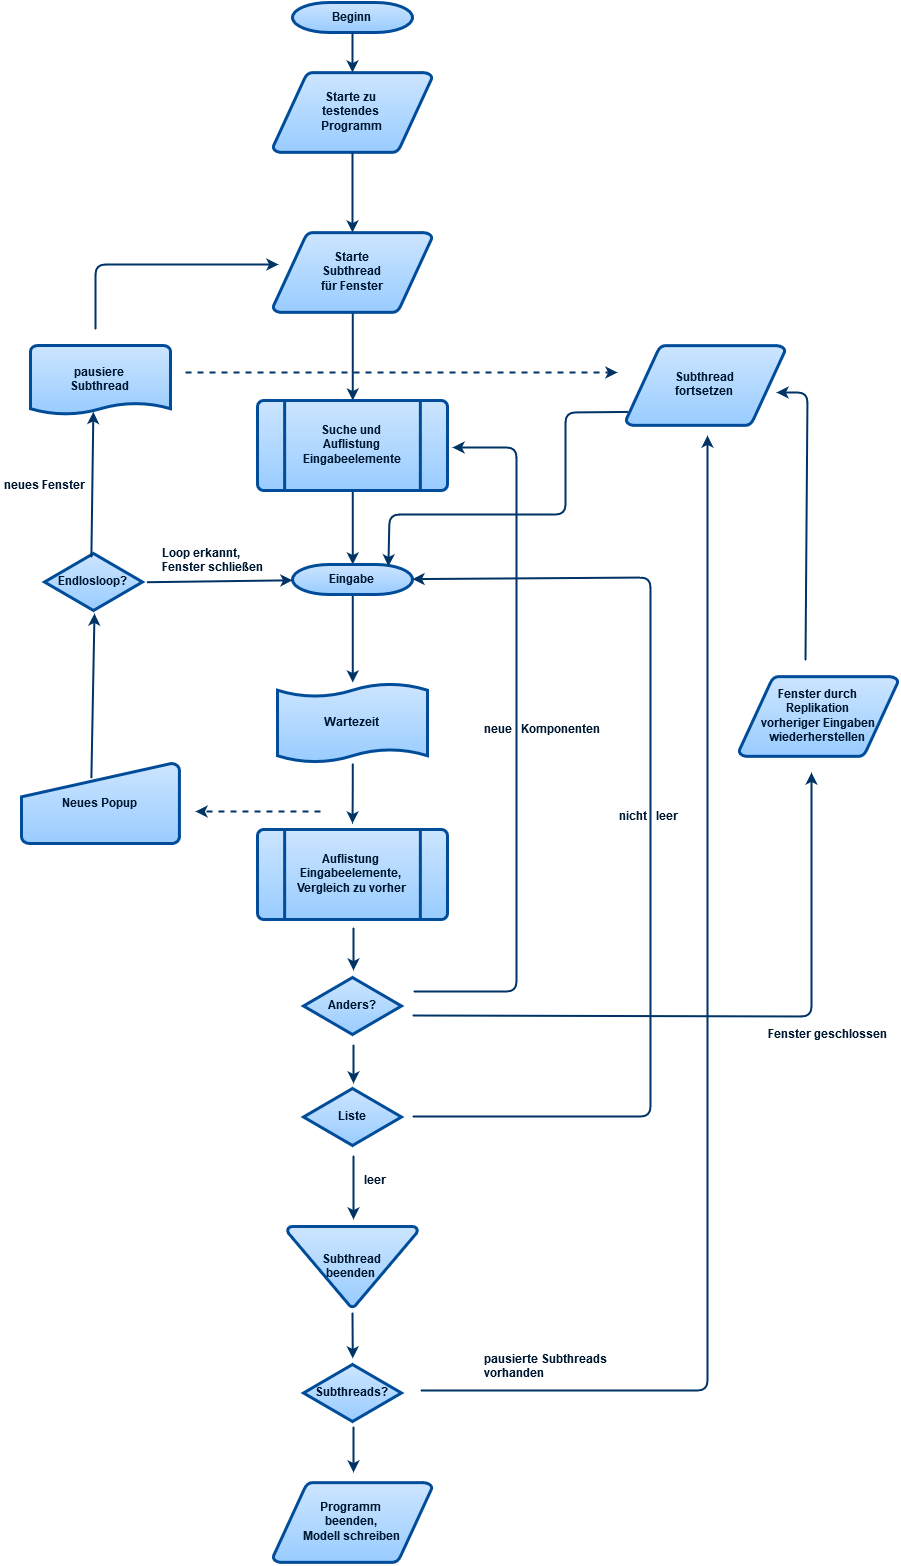
\includegraphics[width=0.85\textwidth]{bilder/autotester.png}
	\caption{Schematischer Ablauf des Autotesters}
	\label{fig:autotesterschematic}
\end{figure}

\begin{algorithm} \SetAlgoLined
	\KwData{Laufender Test $T$, neues Fenster/Popup $P$}
	\KwResult{Alle an $P$ anhängigen Komponenten wurden getestet, Test $T$ setzt fort}
	vorherige Testinstanz $T$ anhalten, sichert Zustand\;
	$Tn \longleftarrow Komponententester(P)$\;
	vorherige Testinstanz $T$ starten, Zustand wiederherstellen\;
	\caption{Popupbehandlung}
	\label{alg:autotesterpopup}
\end{algorithm}

\begin{algorithm} \SetAlgoLined
	\KwData{Wurzelkomponente/Fenster $A$, Liste von Problemstrings $StrL$;}
	\KwResult{Alle an $A$ anhängigen Komponenten wurden getestet}
	Komponentenliste $C: \longleftarrow A$ auf Komponenten durchsuchen\;
	$C$ ein Mal zufällig durchmischen\;
	\For{Komponente $k \in C$}
	{
		\If{$k \in Eingabeelemente$}
		{
			$k \longleftarrow \glqq{}Nutzereingabe\grqq{}$\;
			kurze Wartezeit (um GUI reagieren zu lassen)
		}
		\ElseIf{$k \in Texteingabeelemente$}
		{
			\For{String $s \in StrL$}
			{
				$k \longleftarrow \glqq{}Eintippen\grqq{} StrL$\;
				$k \longleftarrow \glqq{}Bestaetigung\grqq{}$\;
				sehr kurze Wartezeit (um GUI reagieren zu lassen)
			}
			$k \longleftarrow$ \glqq{}Eintippen\grqq{} zufälliges $s \in StrL$\;
		}
		\If{Auftreten neues Fenster/Popup $P$}
		{
			Popupbehandlung($P$)\;
		}
	}
	\caption{Komponententester}
	\label{alg:autotestermain}
\end{algorithm}

\begin{algorithm} \SetAlgoLined
	\KwData{Laufender Test $T$, vorheriger Test $Ta$, Fenster $F$ wurde vor Beendigung des Tests vom Programm geschlossen}
	\KwResult{Test $T$ setzt auf neuem, identischen Fenster $Fn$ fort}
	$Ts \longleftarrow$ laufende Testinstanz $T$ anhalten, sichert Zustand\;
	$T \longleftarrow Ta$, $T$ in Rückwärtslauf schalten\;
	\For{vorherige betätigte Komponente $k \in C(T)$}
	{
		\If{Auftreten Fenster $Fn$ mit $Fn == F$}
		{
			$T$ in Vorwärtslauf schalten\;
			Testinstanz $T$ wieder anhalten, sichert Zustand\;
			$T \longleftarrow Ts$, $F$ mit $Fn$ ersetzen, Zustand wiederherstellen\;
			Diese Suchschleife beenden, $T$ fortfahren lassen\;
		}
	}
	
	\caption{Verhalten bei Verlust des zu testenden Fensters}
	\label{alg:autotesterwindowloss}
\end{algorithm}


\subsection{Herausforderungen bei der Implementation}

Die Implementation des als Konzept vorliegenden Testers erfolgte iterativ
-- es war zu Beginn nicht sichergestellt, dass das Konzept als solches
überhaupt realistisch umsetzbar ist -- und passte sich während des
Entwicklungsprozesses laufend an neue Erkenntnisse und Erfahrungen
mit der Java-Swing-API und ihrem Verhalten an. Insbesondere
die asynchrone Eingabeverarbeitung und die resultierenden Probleme
bei der Verfolgung ihrer Auswirkungen waren eine technische Herausforderung.

Es traten häufig Situationen auf, in denen Ursache und Wirkung nicht
in Zusammenhang gebracht werden konnten. Der Prototyp beendete
Testabläufe vorzeitig oder geriet selbst in einen Fehlerzustand
oder fror ein. Unendliche Schleifen traten beim Testdurchlauf unregelmäßig auf.
Das ursprüngliche strikt deterministische Konzept wurde durch Zufallsdaten
erweitert, da es keine praktikable Alternative gibt, eine praktisch
unbegrenzte Zahl möglicher Schaltzustände zu testen -- gemeint
sind Eingabeelemente, die z.B. über einen AN/AUS Zustand verfügen,
oder eine einzelne Wahl zwischen mehreren Alternativen erfordern.
Fehler des Testers wurden durch die Fehlerabhandung des getesteten
Programms maskiert (und umgekehrt). Es musste ein Format gefunden
werden, durch das unbekannte beliebige Objekte bzw. Elemente aus den Daten
der graphischen Oberfläche für einen Menschen verständlich und prägnant
als Debug-Informationen in einer Konsole dargestellt werden können.

Dieses Format musste dann jeweils beim Auftreten neuer Elementarten
um den kleinsten gemeinsamen Nenner der zugrunde liegenden Klassen
erweitert werden. Für den Tester und damit eventuelle Nutzer von
Interesse sind nämlich nur die Daten, die ein graphisches Element
von seiner Funktion bzw. Bestimmung her von anderen unterscheidet.
Die übliche Implementation der Repräsentation als Zeichenkette
beinhaltet aber eine Anzahl überflüssiger oder irreführender
Informationen, wie z.B. die lokalen Koordinaten auf dem Bildschirm,
die absoluten und relativen Größenangaben der Fenster und ihrer
enthaltenen Elemente, oder nur für die kosmetische Darstellung
relevante Datenfelder.

Die laufende Änderung der sichtbaren graphischen Elemente als Reaktion
auf Eingaben war eine weitere Problematik, die es zu lösen galt.
Da nun ein Verfahren vorlag, um graphische Elemente miteinander
vergleichen zu können, konnte der gesamte an ein Element anhängige Baum
graphischer Elemente vor und nach Durchführung einer Eingabe ausgelesen
und die Ergebnisse miteinander verglichen werden. Es stellte sich heraus,
dass sowohl neue Elemente hinzukommen als auch bestehende Elemente im
Betrieb entfernt werden können. Dies muss vom Tester überwacht und
im Testablauf berücksichtigt werden. Neue zu Eingaben fähige Elemente werden 
an die Liste noch zu prüfender Eingabemöglichkeiten gehängt und
nicht mehr existierende Komponenten aus dieser Liste entfernt. Dies war
auch einer der Gründe für ein nichtdeterministisches Vorgehen:

Da Elemente nachträglich verschwinden können, also bei einem strikt
deterministischen Vorgehen nie getestet werden würden, kann nur ein
Verfahren mit Zufallselementen diese jemals erreichen. Die zufällige
Anordnung der Testreihenfolge stellt sicher, dass jedes durch Nutzung 
bzw. Eingaben in irgendeiner Reihenfolge erreichbares Element
irgendwann auch getestet wird. Dies unterstellt zwar eine unendliche
Anzahl an Testdurchläufen, aber für eine für alle praktischen Zwecke
unendliche Anzahl an möglichen Eingabekombinationen gibt es schlicht
keine Alternative. Auch sie hier erwähnt, dass ein menschlicher Tester
entschieden größere Schwierigkeiten damit hätte, wirklich zufällige
Eingabemuster umzusetzen -- Gewohnheiten beim Umgang mit Computern
und Eingabemasken verzerren das Testbild in Richtung eines eher
wahrscheinlichen Vorgangs, aber das Ziel des Konzepts ist ja gerade,
abseits dieser üblichen Pfade zu agieren.


\section{Problematische String-Eingaben}\label{section:naughtystrings}

Es wird eine online erhältliche, quelloffen gepflegte Liste aus Entwicklerkreisen verwendet, 
die \textbf{Big List of Naughty Strings} \footnote{\url{ https://github.com/minimaxir/big-list-of-naughty-strings }}. Diese enthält unter viele bekannte
Vertreter typischer Fehler oder Lücken bei der Verarbeitung von Zeichenketten in Programmen und
insbesondere auch im Internet. Es finden sich Zeichendarstellungen reservierter Begriffe wie
\glqq{}null\grqq{} oder \glqq{}true\grqq{}, SQL-Befehle, HTML und Javascript, exotische Unicode-Zeichen wie das
\glqq{}zero-width space\grqq{} \cite{unicodezerowidth} oder auch diverse DOS- oder Unix-spezifische
Anweisungen oder Optionen für Kommandozeilen.

Ziel ist es hierbei primär, mögliche durch Lücken in der Zeichenverarbeitung ausgelöste Probleme oder gar
Abstürze des Programms schnell herbeizuführen, damit diese diagnostiziert und behoben werden können.
Dies wird auch als \glqq{}Input Sanitization\grqq{} bzw. Eingabevalidierung bzw. -prüfung bezeichnet. 
Obwohl dieses Verfahren primär zur Verteidigung gegen Skript-Angriffe auf Webseiten dient
\footnote{\url{ http://www.scip.ch/?labs.20110914 }}, 
zählt eine wenig sinnvolle, aber dennoch mögliche Eingabe, 
die das zu testende Programm in der Ausführung beeinträchtigt oder sogar stoppt, klar zur 
Softwarequalität und sollte korrekt behandelt werden. Eine Fehlermeldung an den Nutzer zum
Beispiel ist eine völlig legitime Reaktion, eine unbehandelte Ausnahme dagegen nicht.

Je nach Betriebssystem führen unterschiedliche Symbole und Begriffe z.B. als Datei\-namen
manchmal zu sonderbaren Effekten und Fehlermeldungen oder sind schlicht verboten.
Beispiele hierfür wären \textbf{COM} oder auch von geschweiften Klammern \glqq{}\{\}\grqq{} umschlossene
Begriffe unter Windows, oder \textbf{dev} unter Linux. Programme, die ihre eigenen
Dateioperationen mit wählbaren Dateinamen durchführen, sehen häufig nicht eine vollständige
Behandlung all dieser möglichen Sonderfälle vor, und die Programmiersprache Java erzwingt
trotz vorgegebenen I/O-Ausnahme\-behandlungen nicht, alle Eventualitäten abzudecken.


\section{Zustandserfassung, -sicherung und -verfolgung sowie Kontrollmechanismen}\label{section:statemonitoring}

Um eine Überprüf-, Nachvollzieh- und Reproduzierbarkeit der vom automatischen Tester
durchgeführen Eingaben sicherzustellen, müssen diese bei jedem Testdurchlauf erschöpfend
mitprotokolliert werden. Da die Erstellung eines Modells der zu testenden Anwendung 
ebenfalls als Ziel definiert wurde, bietet sich ein Graph als Datenstruktur an. Die Analogie
eines solchen sowohl zum Java-AWT/Java-Swing-Datenmodell als auch zu den meisten 
Automatendarstellungen der Informatik lässt eine einfache und intuitive Implementation
erhoffen. Auch lassen sich die von einer Applikation geöffneten Fenster als Knoten und die
dorthin führenden Eingaben als Knotenübergänge auffassen, und es existieren
fertige Java-Bibliotheken für normierte Graphdarstellung. Für dieses Projekt genutzt
werden die quelloffene Graphbibliothek \textbf{JGraphT} \footnote{\url{ http://http://jgrapht.org/ }} sowie die
ebenfalls offene Visualisierungsplattform \textbf{Gephi} \footnote{\url{ http://gephi.github.io/ }}.

Sobald man die Frage nach dem \textbf{Wie} beantwortet hat, stellt sich als Nächstes
eine ähnliche nach dem \textbf{Was}. Unglücklicherweise sind Java-Applikationen der realen
Welt nicht nach akademischen Maßstäben gläsern und überschaubar. Kurz nach dem
Start eines konkreten Testdurchlaufs für \textbf{FirstSpirit} durch den Autotester zeigt der
Java-Debugger bereits 20 verschiedene Threads oder Kontrollfäden an, die alle auf
die eine oder andere Weise den Tester oder das Testobjekt beeinflussen können.
Java ist objektorientiert \cite{java7insel}, was im Gegensatz zu den Alternativen 
wie imperativen oder funktionellen Programmen in der Theorie erlaubt, jede laufende 
Instanz eines Programms in einen für Menschen verständlichen Datensatz zu übersetzen.

In der Praxis zeigt sich aber, dass die Masse an Kontrollfäden, Objekten und
sich gegenseitig beeinflussenden Nebeneffekten eine vollständige Zustandserfassung
und -verfolgung äußerst impraktikabel, wenn auch nicht völlig unmöglich, macht.
Das zu testende Programm muss folglich als \glqq{}Black Box\grqq{} verstanden werden.
Obwohl wir technisch in der Lage sind, die Inhalte einzusehen, ist die genaue
Funktion ein Rätsel, und wir können lediglich Rückschlüsse aus beobachtetem
Verhalten ziehen. Für unsere Zustandserfassung heißt dies, dass wir lediglich
die Klasse einer dargestellten Oberflächenelements sowie aus globalen
Schnittstellen erhältliche Informationen nutzen können, um einen beliebigen Zustand
von einem anderen zu unterscheiden. 

Diese Methodik hängt bis zu einem gewissen Grad von der jeweiligen Implementation 
des getesteten Programms ab und ist nicht frei von möglicher Ambivalenz,
insbesondere bei generellen, häufig benutzten Elementen -- wenn aber
das Verhalten eines Objekts von Instruktionen und nicht von Daten abhängt,
gibt es für den Tester keine praktikable Möglichkeit, dies festzustellen
oder ohne Kontext irgendetwas sinnvolles mit der Information anzufangen.

Ein Beispiel hierfür ist im Rahmen des FirstSpirit-Programms die Klasse
\glqq{}SearchDialog\grqq{}. Sie dient der Auswahl einer Datei oder eines Verzeichnisses
des Betriebssystems. Die Klasse beinhaltet keine Datenfelder, die für
eine Identifizierung einer konkreten Instanz hilfreich wären. Sie ist
Unterklasse von \glqq{}SelfDisposingDialog\grqq{}, welches ebenfalls keine Felder
enthält, und schließlich \glqq{}JDialog\grqq{}, eine Basisklasse der Java-Swing-API.
Diese garantiert nun die Präsenz eines Titels für jedwede Instanz
seiner Klassen, selbst wenn dieser nicht definiert oder leer sein sollte.
Worin unterscheiden sich nun verschiedene Instanzen von \glqq{}SearchDialog\grqq{}?

Die Antwort ist leider: In den Anweisungen, die an die Schnittstellen
des jeweiligen Objekts geschrieben wurden. Wir können dazu auf einen
aussagekräftigen, eindeutigen Titel des Suchfensters hoffen. Die
Anweisungen lesen und vergleichen zu wollen wäre zwar theoretisch
möglich, aber praktisch nutzlos. Die Instanz ist von Ihrem Nutzungskontext
abhängig, und Kontext ist etwas, dass der Autotester nicht verstehen kann.
Lediglich die Eingaben, die zu dem Suchfenster geführt haben,
lassen weitere Rückschlüsse darauf zu, wofür es dienen könnte.

Für den Autotester und eine für Menschen verständliche Protokollierung
wurde die Lösung einer eigenen \textbf{toString()} Methode gewählt.
Hierbei nimmt der Tester ein beliebiges darstellbares Objekt aus dem Testprogramm,
vergleicht es mit einer Reihe von der Java-Swing-API vorgegebenen
Objekten und Schnittstellen, und wählt eine passende Textdarstellung aus.
Üblicherweise ist dies der \glqq{}simple Classname\grqq{}, der einfache Klassenname,
da dieser nach gängigen Java-Konventionen den Nutzen einer Klasse zumindest
andeutet, kombiniert mit den möglicherweise vorhandenen kritischen Daten
der spezifischen Typklasse. Im Falle eines Fensters beispielsweise wäre
dies die Zeichenkette, die in der Titelzeile angezeigt wird. Im Fall
eines beschrifteten Knopfes die Beschriftung. Im Fall eines Knopfs
nur mit Glyphe oder Icon, ohne jegliche Beschriftung, 
ziehen wir den \glqq{}Tooltip\grqq{} bzw. Nutzungshinweis heran,
die vom Programmierer vorgesehene helfende Zeichenkette, die angezeigt
wird, wenn der Nutzer seinen Mauszeiger kurz über das betreffende Symbol hält.
Wir verlassen uns also auf gängige Programmierpraxis sowie Eigenarten der 
Java-Datenstrukturen, um ähnliche Instanzen zu identifizieren.

Zur Verfolgung des Programmzustands kann entsprechend nur die Liste
bzw. das Protokoll vergangener Eingaben an Elemente der Oberfläche
herangezogen werden. Um einen bestimmten Zustand zu reproduzieren,
ist die einzig sichere Lösung, alle dahin führenden Schritte nachzuahmen.
Es ist zwar häufig möglich, auch auf einem direkteren Weg zu einer
vermuteten Fehlerstelle zu gelangen, aber es muss immer damit gerechnet
werden, dass ein bestimmter Fehler nur bei perfekter Reproduktion
einer gewissen Eingabekette auftritt. 

Die Schwierigkeit beim
Verfolgen des Zustands der Java Virtual Machine verhindert
gleichzeitig auch das Einfrieren oder Abspeichern eines bestimmten Zustandes
zwecks späterer Wiederherstellung. Java sieht überhaupt nicht vor,
den gesamten Systemzustand sichern und laden zu können. Eine dennoch
denkbare Möglichkeit ist die Verkapselung des Testsystems in einer
virtuellen Umgebung, die beliebig pausiert, gespeichert und geladen
werden kann. Dies ist aber enorm aufwändig und würde zumindest eine
Kommunikation zwischen virtuellem System (bzw. einer Kontrolleinheit
ausserhalb desselben) und des darin laufenden Tests erfordern.
Auch ist der Speicher- und Ladevorgang selbst nicht unaufwändig,
da ein komplettes modernes Betriebssystem als Speicherabbild zumindest einige hundert
Megabyte an Informationen umfasst.

Virtualisierung ist dennoch ein guter Ansatz, um die Tests
durchzuführen. Da der Ablauf selbst nichtdeterministisch ist,
spricht nichts dagegen, eine Vielzahl von Testinstanzen parallel ablaufen zu
lassen. Man muss nur beachten, dass zu viele parallele Instanzen den VM-Host
so stark belasten können, dass die vom Tester eingelegten Pausen
zwischen Eingaben nicht mehr ausreichen könnten, um die jeweilige graphische
Oberfläche reagieren zu lassen. Dies würde eine korrekte Verfolgung
der aus Eingaben erfolgten Reaktionen zumindest sehr schwierig,
wahrscheinlich sogar unmöglich machen.


\subsection{Repräsentation der Programmzustände als Graph}

Eine eigene Graphimplementation für das Projekt zu verfassen wäre
außerhalb des Rahmens, daher wurde nach einem möglichst verbreitetem
Datenstandard und passenden Bibliotheken gesucht. Die Wahl fiel auf
die quelloffenen Projekte der Graphbibliothek \textbf{JGraphT} \footnote{\url{ http://http://jgrapht.org/ }} 
sowie der Visualisierungsplattform \textbf{Gephi} \footnote{\url{ http://gephi.github.io/ }}.
Das gewählte Datenformat ist \textbf{.graphml} \footnote{\url{ http://graphml.graphdrawing.org/specification.html }}.
Es handelt sich hierbei um einfache Textdateien im \textbf{xml}-Format,
welche auch menschlich noch lesbar und verständlich sind, und notfalls
auch editiert oder korrigiert werden könnten. 

Innerhalb des Testers erstellt JGraphT während des Testvorgangs 
ein Datenmodell des Graphen der getesteten Applikation. Nach erfolgreichem
Abschluss desselben wird das Resultat in besagtem graphml-Format
in einer eindeutig nach dem Testdatum benannten Datei abgespeichert.
Diese Datei ist dann zwar vollständig und auch von Menschen lesbar,
aber noch absolut undurchsichtig. Visualisierung ist notwendig,
um die Informationen in eine verständliche Form zu bringen.
Hierzu wird wahlweise Gephi verwendet. Es öffnet graphml-Dateien
und erlaubt die automatische Neuanordnung eines Graphen auf dem
Bildschirm, um maximale Ansehnlichkeit zu erzielen.

Nach einigen Probeläufen erwies sich der in Gephi mitgelieferte 
Yifan-Hu-Algorithmus \cite{hu2005efficient} als gut geeignet,
um einen komplexen Graph sternförmig auszubreiten. Ein beispielhaftes
Ergebnis lässt sich auf Seite \pageref{fig:model_firstspirit_notext}
begutachten. In der Grundeinstellung werden die von GraphT
abgespeicherten Knotendaten bzw. Programmzustände nicht angezeigt.
Diese relativ umfangreichen Zeichenketten erfordern für eine minimale
Lesbarkeit noch manuelles Verschieben und Sortieren der Graphknoten.
Ist dies aber erfolgt, erhält man aus dem Durchlauf eines blind testenden
Programms aber tatsächlich eine deckende Abbildung der getesteten
Applikation bzw. Ihrer möglichen Fensterdarstellungen. Zu sehen
ist ein solches finales Resultat auf Seite \pageref{fig:model_freespirit_06.10.2015}.

Einige Anmerkungen zu diesen Bildern: Der Knotensortieralgorithmus
nimmt auf die in diesem Fall ungewöhnlich langen Beschriftungen der einzelnen
Knoten keine Rücksicht. Für eine irgendwie lesbare Darstellung müssen die
Graphen nach der automatischen Sortierung noch per Hand verschoben werden,
bis keine Texte mehr überlappen. Ein weiteres Zugeständnis an Lesbarkeit
ist die Darstellung von Eingaben bzw. betätigter Schaltflächen als
Knoten. Eigentlich sollten Knoten nur Zustände darstellen, Eingaben
sind die Kanten bzw. Übergänge zwischen Zuständen. Dies führt aber dazu,
dass die langen Texte der Eingabedarstellungen an den Kanten dargestellt
werden, die nicht beliebig verschoben werden können. Sie liegen immer
zwischen zwei Knoten. Eine vernünftige Darstellung in dieser Form
erwies sich als unmöglich. Wenn die Eingaben ebenfalls als Knoten
dargestellt werden, können sie in der Darstellung beliebig verschoben
werden, sodass auch ihre Texte nicht überlappen und tatsächlich
gelesen werden können.


\section{Minimale Nichtautomatische Angaben}

Das Ziel eines vollautomatischen Tests kann leider nur annähernd erreicht werden,
wenn gleichzeitig andere Anforderungen wie \glqq{}Die Testzeit ist nicht unendlich lang\grqq{}
in Betracht gezogen werden müssen. Um auch die gewünschte graphische Oberfläche zu
testen und einige Fallstricke zu vermeiden, bietet der Autotester eine Konfigurationsdatei
nach dem Java \glqq{}Properties\grqq{} Standard, in der einige Angaben gemacht werden können bzw. müssen:

\begin{itemize}
  \item \textsc{targetGUISimpleClassName} der Klassenname der zu testenden Oberfläche
  \item \textsc{testStartDelayInSeconds} eine kurze Pause nach dem Start der Oberfläche, um Ladezeiten zuzulassen
  \item \textsc{blackListedAbstractButtons} nach dem Benennungs-Prinzip des Autotesters definierte unantastbare Standard-Schaltflächen
  \item \textsc{blackListedWindowKeywords} nach dem Benennungs-Prinzip des Autotesters definierte ignorierte Fenster
  \item \textsc{blackListedComponentsSimpleClassNames} nach dem Benennungs-Prinzip des Autotesters definierte unantastbare Eingabeelement-Klassen
  \item \textsc{sleepTimeMillisTextfieldEntries} Dauer der Wartezeit zwischen Texteingaben
  \item \textsc{sleepTimeMillisBetweenFakeMouseClicks} Dauer der Wartezeit zwischen Mauseingaben
  \item \textsc{modelOutputFolder} Absoluter Ordnerpfad im Dateisystem, in dem die Resultate gespeichert werden sollen
\end{itemize}

Diese Angaben genügen, um für das sehr komplexe FirstSpirit-Programm einen regelmäßig annähernd
vollständigen Testdurchlauf über alle existierenden Schaltflächen zu ermöglichen.
Die gewählte Zeit vor dem Testbeginn sind zehn Sekunden. FirstSpirit ist eine sehr umfangreiche,
vernetzte Applikation. Als unantastbare Schaltflächen definiert wurden der globale Knopf
zum Beenden von FirstSpirit, ein Knopf, der zum Start eines externen Internetbrowsers führt
(nicht Bestandteil des Tests), der Knopf, der in Standard-Dateiauswahlfenstern das Erstellen eines neuen
Ordners ermöglicht (wäre als Standard-Ausnahme vermutlich sogar sinnvoller), sowie drei
Debug-Schaltflächen, die die Logdatei des Testablaufs mit den Ausgaben des Programms selbst
überschwemmen können.

Als einziges ignoriertes Fenster wurde die \glqq{}FirstSpirit Zwischenablage\grqq{} definiert. Durch eine
Eigenart in der Implementation sind die resultierenden Fenster technisch gesehen immer neuartige
Instanzen, was zu einem unendlichen Test führt, da der Tester alle Fenster testen will.
Eine unendliche Anzahl von Fenstern führt leider auch zu einer unendlichen Anzahl an Tests.
Aus Effizienzgründen wurden als nächstes zwei häufig auftretende Klassen von Tests ausgeschlossen,
welche zwar technisch gesehen Eingaben erlauben, aber im FirstSpirit-Programm lediglich
darstellende Funktion haben. Dabei handelt es sich um \glqq{}GlowLabel\grqq{} und \glqq{}SynthScrollBarUI\grqq{}.
Für die eingestellten Pausen zwischen Text- und Mauseingaben haben sich zehn und 2000 Millisekunden
als geeignet herausgestellt. Dies hängt aber stark vom System ab, auf dem der Test durchgeführt wird,
und insbesondere der Auslastung des Systems. Wenn von einer virtualisierten Umgebung ausgegangen
wird, von der viele Instanzen parallel ablaufen, wäre es vermutlich sehr sinnvoll, diese
Pausen erheblich länger andauern zu lassen.

Zusätzlich zu diesen wenigen Angaben muss natürlich das Testprogramm auch in der Lage sein,
die zu testende Oberfläche als Unterprozess zu starten. Nur so kann der notwendige Zugriff
auf die Daten der laufenden Applikation erfolgen. Würde man zunächst das zu testende
Programm starten, und dann den Tester, wären beide in verschiedenen JVM-Instanzen
verkapselt, die jeweils keinen Zugriff aufeinander zulassen. Für einen solchen
Start als Unterprozess ist die Startklasse der zu testenden Applikation notwendig,
diese kann aus den Metainformationen einer lauffähigen Java \glqq{}JAR\grqq{}
ausgelesen werden. Zusätzlich bieten sich verschiedene Parameter bzw. Argumente
für die JVM an, die z.B. zusätzliche Speicherallokation oder einen anderen
Algorithmus für den Garbage Collector erlauben. Auch ist es bei gewissen Anwendungen,
darunter FirstSpirit, möglich, direkt im Programmstart Parameter wie Login-Daten
oder Programmports zu spezifizieren, um eine Testblockierende Login-Maske
zu überspringen.

Alternativ hätte ein System vorgesehen werden können, welches gewisse Eingaben
bei einem definierten Eingabefeld vorschreibt. Dies wäre für maximale Kompatibilität
hilfreich, wenn ein Programm solche Kommandozeilen-Parameter nicht zulässt.
In diesem Fall hat es sich aber als unnötig erwiesen. Es sei auch die
Annahme in den Raum gestellt, dass nur Entwickler diese Testapplikation
verwenden werden, also in jedem Fall Zugriff auf Quellcode besteht,
und ein entsprechendes Feature relativ schnell und einfach an bestehende
Applikationen angefügt werden kann. Wenn nicht -- der Autotester selbst
wird vermutlich quelloffen verfügbar sein, und eine Implementation
dieser Idee kann von interessierten Parteien umgesetzt werden.


\subsection{\glqq{}minimale\grqq{} Angaben in der Praxis}

In der weitergehenden Nutzung des Autotesters mit verschiedenen
Programmen wurde klar, dass eine gewisse Anpassungs- oder
Lernzeit des Programms mit dem Testsubjekt zwingend notwendig ist.
Über die Definition des Anwendungsfensters hinaus müssen für
effiziente Durchläufe in jedem Fall die Schaltflächen, die Beendigung
des jeweiligen Programms resultieren, auf die Blacklists gesetzt
werden. Darüber hinaus hat jedes getestete Programm eine oder
mehrere Eingaben oder Fenster, die in einem unendlichen oder
sonst unbrauchbaren Durchlauf resultierten -- es wäre vermutlich
eine gute Idee, den Tester um eine maximale Laufzeit oder
eine maximale Prüftiefe oder etwas Ähnliches zu erweitern.

Auch müssen eventuelle Abstürze des getesteten Programms
abgefangen oder verhindert werden. Unerwartetes Beenden
der Abwendung macht die gewonnenen Erkenntnisse abseits
der Konsole unbrauchbar, da eigentlich auf einen
vollständigen Graphen sowie eine Logdateie hin gearbeitet wurde.
Eine Methodik, die auch Logdateien von unerwartet beendeten
Durchläufen sichert, wäre sinnvoll. In der Praxis läuft
die Nutzung der Autotesters nun so ab, dass ein Entwickler
zunächst die Startklassen und Umgebungsvariablen einrichtet
sowie das Anwendungsfenster der zu testenden Applikation
angibt. Der Autotester leistet hierbei Unterstützung, er
gibt die für ihn sichtbaren Anwendungsfenster an. Anschließend
lässt der Entwickler den Autotester laufen, bis sich die Anwendung
selbst beendet oder unerwartet beendet wird, liest die Logdatei
um den Grund bzw. die ausschlaggebende Eingabe zu ermitteln,
und setzt evtl. ein Fenster oder eine Komponente auf die
Blacklist in der Konfigurationsdatei. Er passt gleichzeitig
die Wartezeiten zwischen den Eingaben an die allgemeine
Verarbeitungsgeschwindigkeit der Anwendung auf dem jeweiligen
Computer an. Je nach Anwendung sind hier nun viele oder
sehr wenige Angaben nötig, um konsistent volle Durchläufe
zu ermöglichen. FirstSpirit hat neun Einträge
in seiner Konfigurationsdatei, jEdit und yEd haben beide
acht. Tendenziell sind allerdings bei yEd die meisten Eingaben
und Fenster vom Test ausgeschlossen, da zwischenzeitlich
partielle Angaben für den Ausschluß implementiert und auch
direkt genutzt wurden.

%%% TeX-master: "../main.tex"
% kapitel5.tex
\chapter{Konkret getestete Applikationen}\label{chapter:concretetests}


Dieses Kapitel stellt nun einige Ergebnisse, die mittels des nach dem Konzepts tatsächlich
implementierten vollautomatischen GUI-Crawler und -Tester erzeugt wurden.
Als erstes getestetes Programm dient hierbei eine Enwicklerversion der von der
\textbf{e-Spirit AG} entwickelten Software \textbf{FirstSpirit} 
\footnote{\url{ http://www.e-spirit.com/de/produkt/arbeiten-mit-firstspirit/usability-fuer-redakteure/ }},
Version 5.2 DEV 201. Entwicklerversionen dieser Software enthalten zusätzliche,
dem normalen Nutzer unzugängliche Schaltflächen und Funktionen.

Als zweite Applikation wurde der beliebte Texteditor \textbf{jEdit}
\footnote{\url{ http://www.jedit.org/ }} gewählt. Die dritte ist
die Java-Graphvisualisierungssuite \textbf{yEd}
\footnote{\url{ http://www.yworks.com/products/yed }}.



\section{Resultate FirstSpirit}\label{section:testresults}

Wie in den Graphdarstellungen auf Seiten \pageref{fig:model_firstspirit_notext} und 
\pageref{fig:model_freespirit_06.10.2015} zu sehen ist, enthält diese Version von
FirstSpirit etwa 34 einzigartige Fenster bzw. Zustände. Sie gehen fast alle vom
Hauptfenster des Programms bzw. dem Zustand zu Beginn des Tests aus,
nur einige wenige sind dahingegen tiefer abzweigend. Die Zahl einer im
Laufe eines vollen Durchgangs betätigter Eingabeelemente liegt im Vergleich bei
über 800. Dies legt nahe, dass umfangreiche interne Zustandsänderungen
möglich sind, die nicht direkt in von außen sichtbaren geänderten
Programmzuständen resultieren. Oder auch, dass eine Menge Eingabeelemente
existieren oder als solche erkannt wurden, deren Betätigung kein messbares
Resultat hatte.

Bedenkt man die Natur von FirstSpirit, ist dies keine große Überraschung.
FirstSpirit ist ein Content Management System bzw. CMS, im Grunde also
ein Client bzw. Editor für Webinhalte. Da der Autotester lediglich den Editor testet,
ohne Rücksicht auf die Inhalte nehmen zu wollen oder auch zu können,
hat die Mehrzahl der getätigten Eingaben keinen für das Konzept erkennbaren
Effekt. Änderungen am editierten Projekt haben aber für den Editor durchaus
-- wie auch immer geartete -- langfristige Konsequenzen, und es ist für
einen produktiven Einsatz des Autotesters anzuraten, solche von Seiteneffekten
beeinflussten Daten vor jedem Testdurchlauf wieder auf einen ursprünglichen
Zustand zurückzusetzen.

Nach Dutzenden von Testdurchläufen auf einem nie zurückgesetzten System
ist das von der e-Spirit AG genutzte Beispielprojekt \glqq{}Mithras\grqq{}
erheblich beschädigt. Zufällige Betätigung diverser Löschbefehle hat
Elemente aus dem Projekt entfernt bzw. Verknüpfungen gelöscht, die für
eine korrekte Funktion spezifischer Bestandteile nötig wären. Obwohl
dies natürlich Auswirkungen auf das Testverfahren hat, zeigt sich doch,
dass dennoch in etwa dieselbe Anzahl von Eingabeelementen getestet wird,
die graphische Oberfläche also nicht zwangsläufig auf ein korrekt funktionierendes
geladenes Projekt angewiesen ist, um alle möglichen Eingaben auszuprobieren.

In einer Produktivumgebung würde der Autotester folgendermaßen integriert:
Im Gegensatz zu Unit-Tests mit JUnit können keine festen Maßstäbe angelegt
werden, nach denen eine Version des Quellcodes zulässig ist oder auch nicht.
Korrektheit ist nicht das erklärte oder auch nur erreichbare Ziel.
Der Autotester wäre dementsprechend nicht im regulären automatischen
Build-Prozess enthalten (und diesen irgendwie anhalten oder behindern),
sondern wäre parallel angeordnet und kontinuierlich oder nach Wunsch
Tests durchführen. Man könnte sich z.B. vorstellen, dass eine neue
Programmversion jeweils fünfhundert (die Zahl ist völlig arbiträr) Durchläufe
des Autotesters auslöst und erfahren soll. Jede Instanz des Testprogramms wird
in einem virtualisiertem System gestartet, in das man vorher die
zentral gelagerte Konfigurationsdatei sowie die nötigen Voraussetzungen
kopiert hat -- in diesem Fall wäre dies das FirstSpirit-Programm sowie
die Dateien des Mithras-Projekts.

Die Logdateien und Ergebnis-Graphen jeder Instanz würden dann wieder zentral
gesammelt und könnten dann auf Gemeinsamkeiten und Abweichungen untersucht
werden. Instanzen, die nicht korrekt beendeten, sind natürlich von besonderem
Interesse. FirstSpirit hat eine eigene Schnittstelle, um Fehlerberichte von
aufgetretenen Ausnahmen weiterzureichen. Diese Berichte sowie in den Logdateien
erwähnte Fehlermeldungen könnten dann von Entwicklern genutzt werden, um
Schwachstellen im Code auszumerzen, wenn diese denn tatsächlich vorliegen.
Idealerweise ist es dem Autotester irgendwann unmöglich, Fehlermeldungen
oder Ausnahmen herbeizuführen, da die Entwickler jede ursprünglich 
unvorhergesehene Eingabe oder -sequenz abfangen oder korrekt behandeln.


\begin{sidewaysfigure}
	\centering
	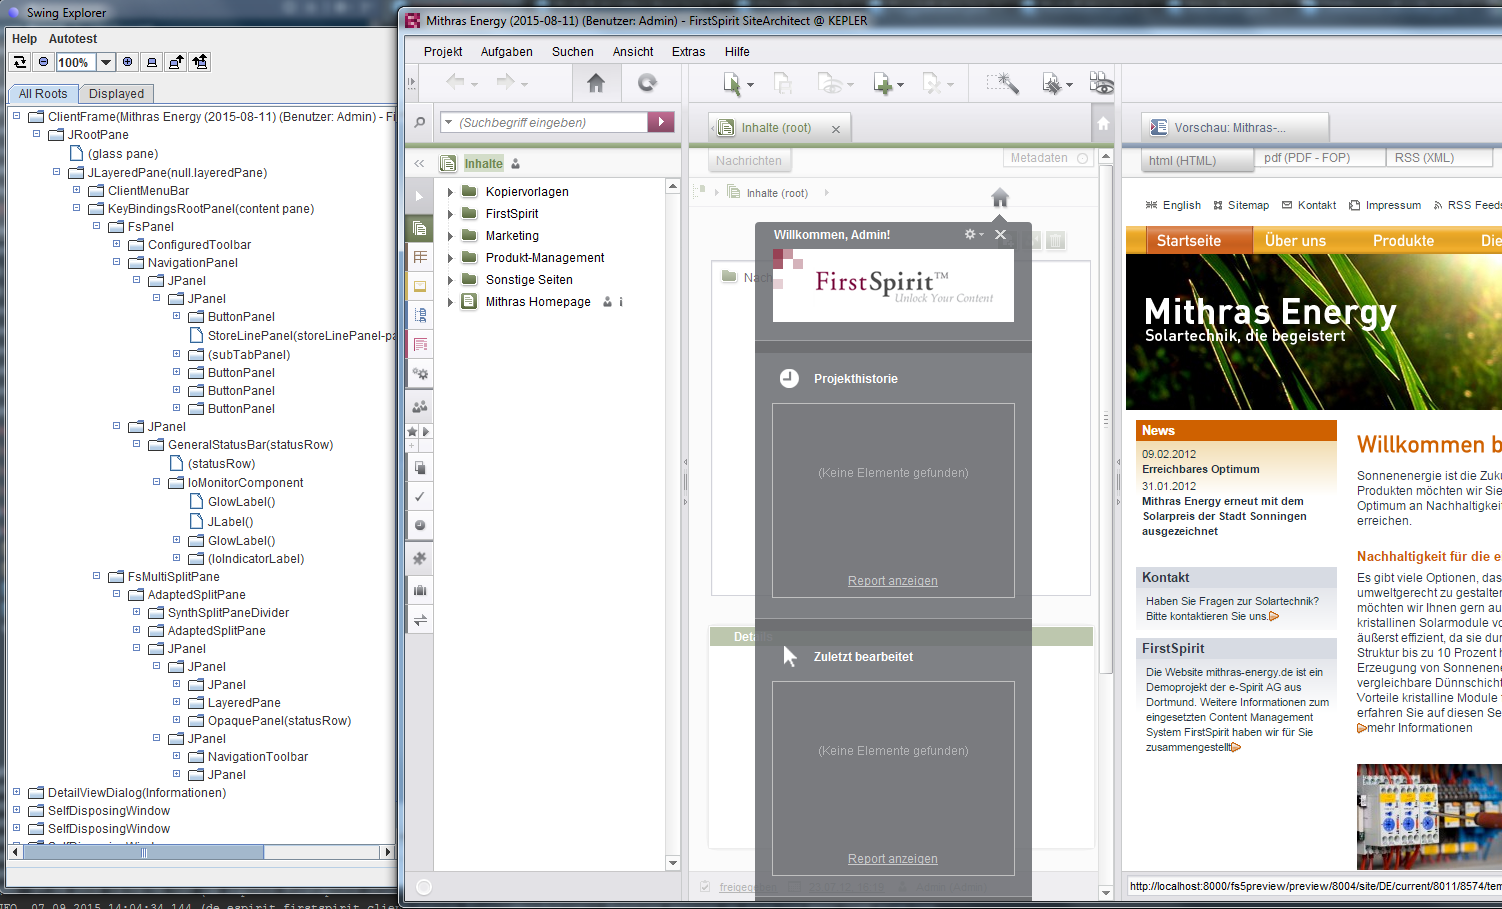
\includegraphics[width=0.85\textwidth]{bilder/screenshot_freespirit.png}
	\caption{Screenshot der e-Spirit CMS-Anwendung FirstSpirit
	sowie anhängigem Swing Explorer, der den Komponentenbaum der Applikation darstellt}
	\label{fig:screenshot_freespirit}
\end{sidewaysfigure}

\begin{figure}
	\centering
	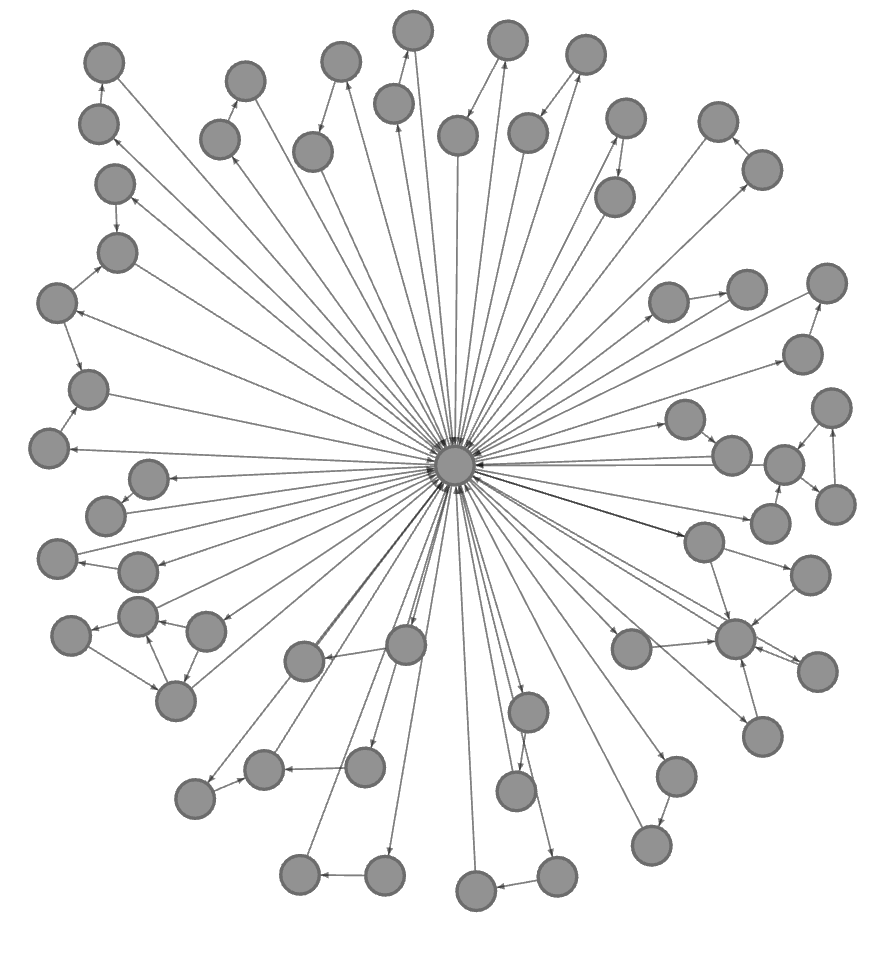
\includegraphics[width=0.85\textwidth]{bilder/model_firstspirit_notext.png}
	\caption{mit Gephi und dem Yifan Hu Algorithmus \cite{hu2005efficient}
    sowie noch für Lesbarkeit maneull angepasste visualierte Graphausgabe 
	des Autotesters über FirstSpirit, hoher Zoomfaktor, keine Beschriftungen.
	Die Pfeile des gerichteten Graphen sind so sichtbar.}
	\label{fig:model_firstspirit_notext}
\end{figure}

\begin{sidewaysfigure}
	\centering
	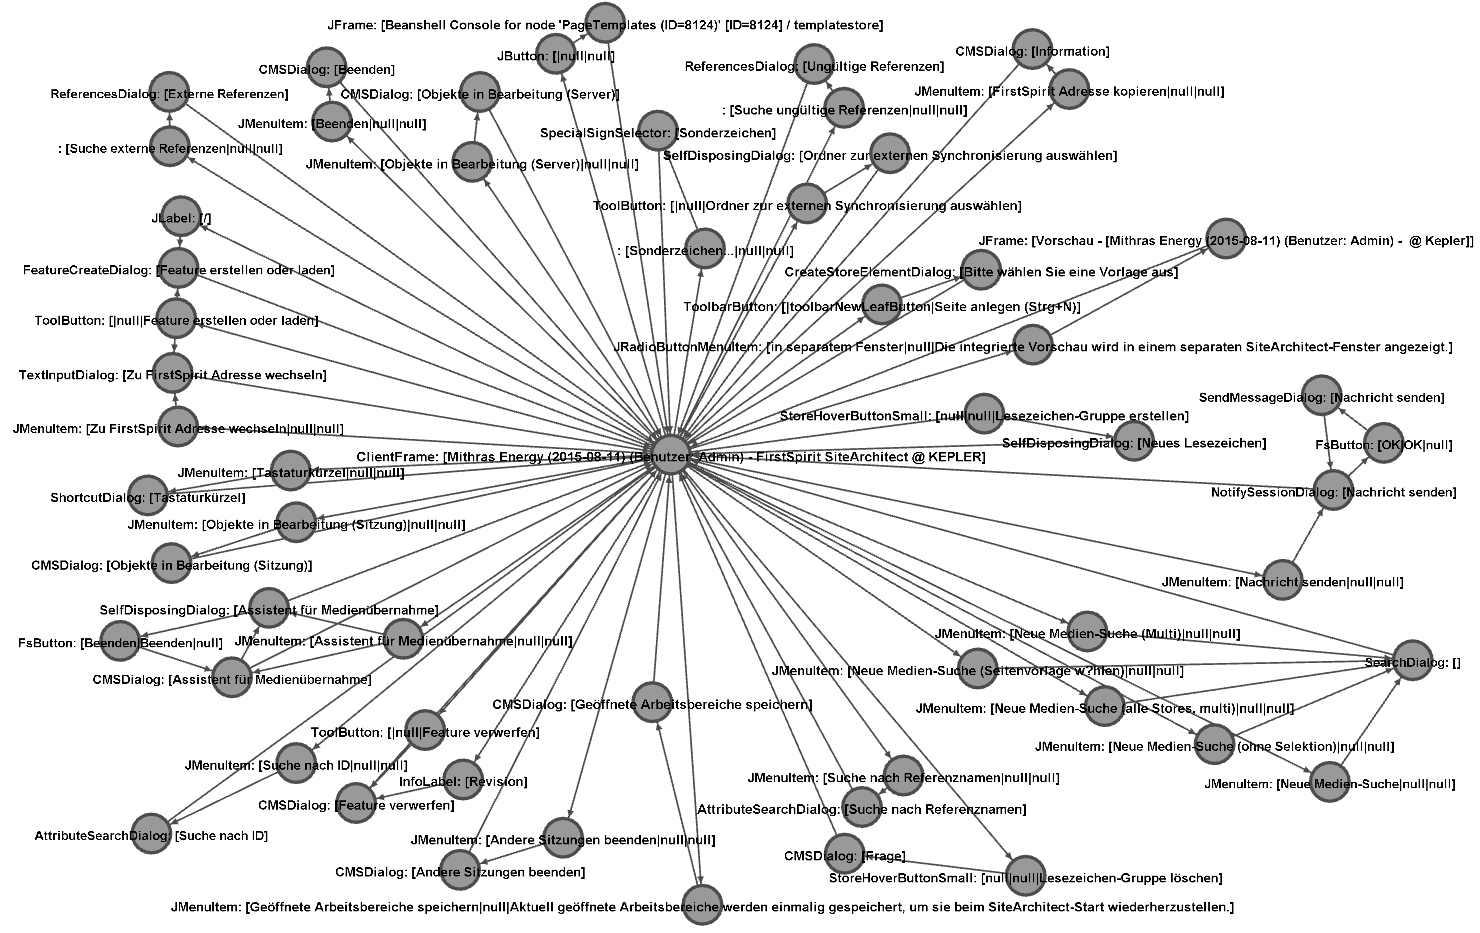
\includegraphics[width=0.85\textwidth]{bilder/model_freespirit.png}
	\caption{mit Gephi und dem Yifan Hu Algorithmus \cite{hu2005efficient}
    sowie noch für Lesbarkeit maneull angepasste visualierte Graphausgabe 
	des Autotesters über FirstSpirit bei einem der ergiebigeren Durchläufe.
	Beschriftungen der Knoten sind aktiviert.}
	\label{fig:model_freespirit_06.10.2015}
\end{sidewaysfigure}



Die Knoten sind in Dreiergruppen angeordnet: Ein Ursprungsfenster, ein Übergangsknoten
(bzw. ein Wort des Modells), sowie der resultierende Zustand bzw. das sich öffnende Fenster.
Dies ist schlicht eine Frage der Lesbarkeit -- anstelle der mittleren Knoten für Übergänge sollten
eigentlich einfach beschriftete Kanten benutzt werden, aber dies schränkt die Möglichkeiten,
den anhängigen Text in eine lesbare Form zu bringen, zu stark ein. Es ist schlicht zu viel
Textinformation, um mit einer Legende o.Ä. auszukommen.


\section{Resultate jEdit}\label{section:testresultsjedit}

Die Wahl für einen zweiten Test fiel auf jEdit
in der neuesten erhältlichen Version 5.3.0,
da der \glqq{}Texteditor für Programmierer\grqq{}
ebenfalls über die benötigte Swing-GUI verfügt und 
durch langjährige Entwicklung bedingt im klassischen
Sinne vermutlich relativ fehlerfrei ist. Eine wenig getestete und daher fehlerträchtige
Applikation ließe keinen vernünftigen Autotest zu, da der Entwickler (oder in diesem Fall
Testentwickler) laufend Probleme bzw. Abstürze im Programm beheben müsste, bis ein vollständiger
Durchlauf und eine Modellbildung möglich wird. Tatsächlich erwies sich jEdit als
dem Testdurchlauf gewachsen -- es wurden zwar nicht abgefangene Ausnahmen produziert,
aber das Programm selbst blieb bei Ausnahmebehandlung durch den Tester lauffähig
und geriet auch in keine Endlosschleifen o.Ä..


\begin{figure}
	\centering
	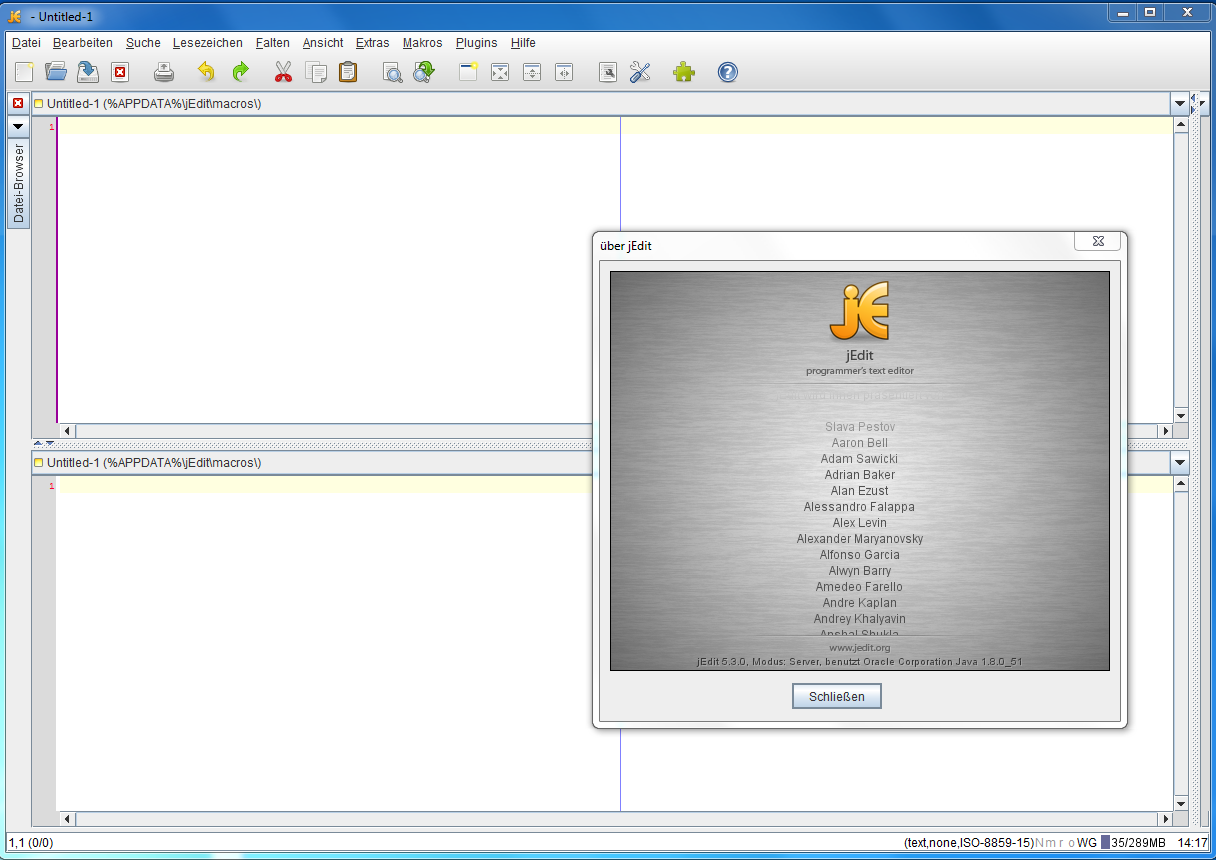
\includegraphics[width=0.85\textwidth]{bilder/jedit_beispiel.png}
	\caption{Screenshot der Java-Applikation jEdit}
	\label{fig:screenshot_jedit}
\end{figure}

\begin{figure}
	\centering
	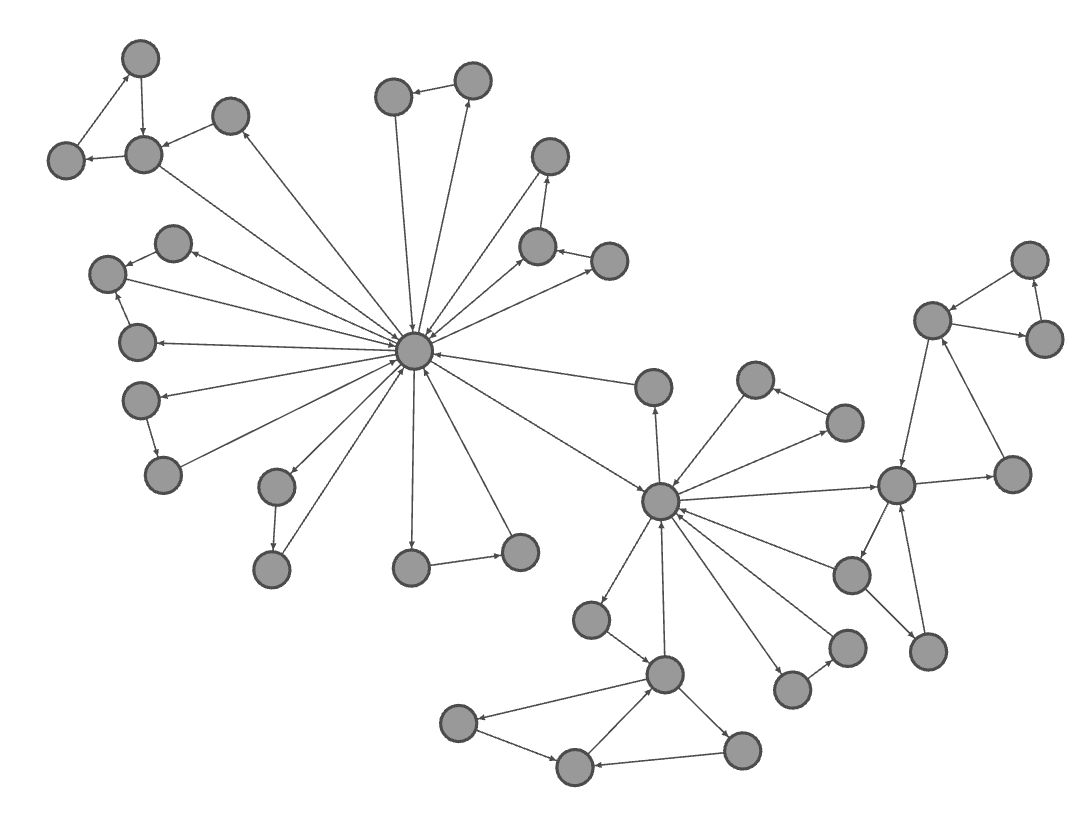
\includegraphics[width=0.85\textwidth]{bilder/model_jedit_notext.png}
	\caption{mit Gephi und dem Yifan Hu Algorithmus\cite{hu2005efficient}
    sowie noch für Lesbarkeit maneull angepasste visualierte Graphausgabe 
	des Autotesters über jEdit, hoher Zoomfaktor, keine Beschriftungen.
	Die Pfeile des gerichteten Graphen sind so sichtbar.}
	\label{fig:model_jedit_notext}
\end{figure}

\begin{sidewaysfigure}
	\centering
	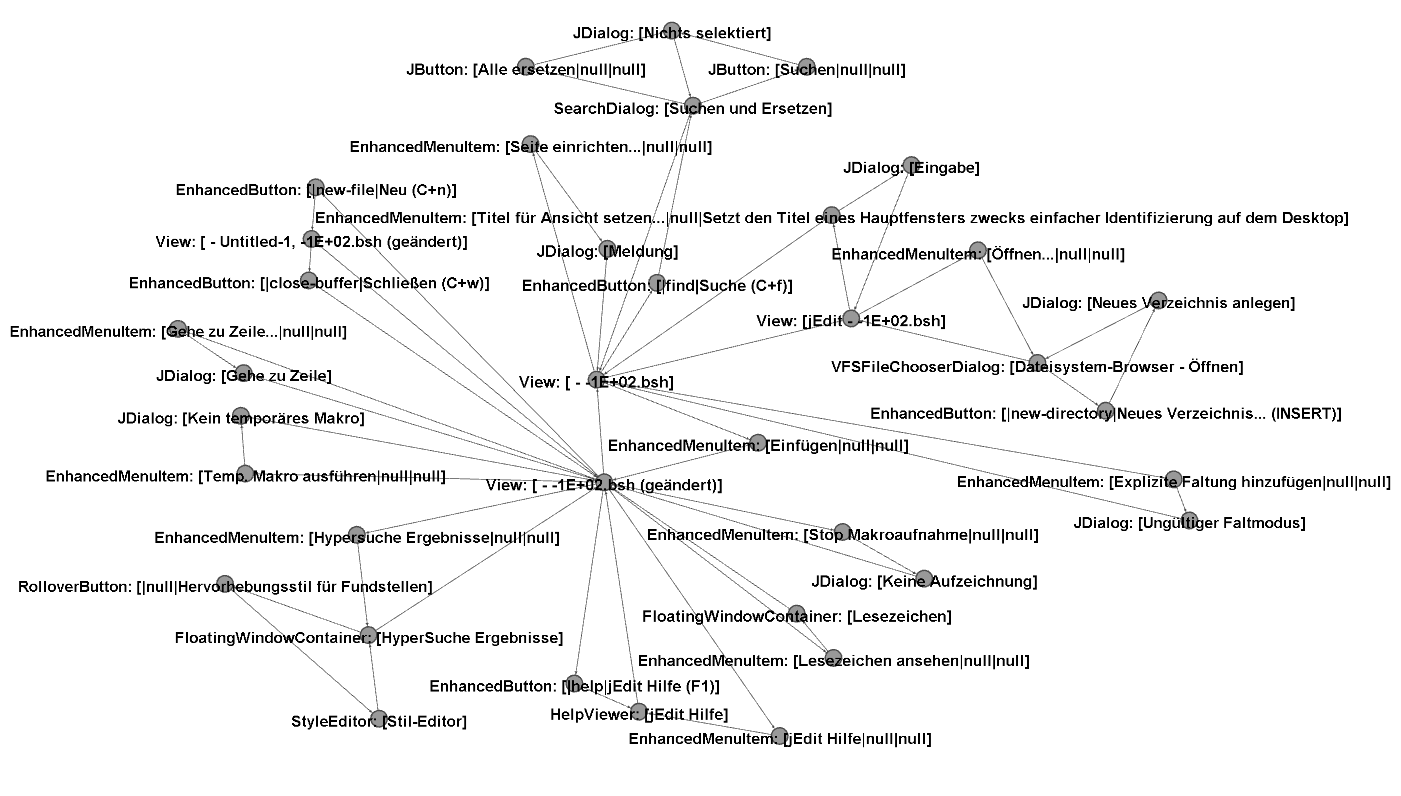
\includegraphics[width=0.85\textwidth]{bilder/model_jedit.png}
	\caption{mit Gephi und dem Fruchterman Reingold Algorithmus\cite{SPE:SPE4380211102}
    sowie noch für Lesbarkeit maneull angepasste visualierte Graphausgabe 
	des Autotesters über jEdit. Beschriftungen der Knoten sind aktiviert.}
	\label{fig:model_jedit}
\end{sidewaysfigure}


Beim Testen von jEdit fielen gewisse Überanpassungen des Autotesters an e-Spirit auf,
welche für eine Entwicklung entlang dieses Programms nicht sonderlich unerwartet
waren. So sah die Konfigurationsdatei beispielsweise nicht vor, Einträge der 
ignorierten Komponenten komplett frei zu lassen. Dies wurde implementiert.
Ebenso fiel auf, dass zwar Zustandsänderungen in Form von sich öffnenden Fenstern
korrekt behandelt wurden, jEdit aber den Zustand des Hauptfensters selbst
ändern kann -- dies würde in FirstSpirit auch passieren, wenn der Tester in der
Lage wäre, das Projekt zu wechseln. (Bei einer unendlich langen Testreihe
wird er dies irgendwann hinbekommen, aber so viel Zeit haben wir nicht)
Der Tester wurde mit Hinblick auf mögliche interne Zustandsänderungen
des aktuell getesteten Fensters erweitert und nimmt dies nun korrekt in
das Modell auf.

Zu sehen ist dies z.B. im Modell von jEdit[\ref{fig:model_jedit}]
auf Seite \pageref{fig:model_jedit} oder im textfreien Fall
[\ref{fig:model_jedit_notext}] auf Seite \pageref{fig:model_jedit_notext}.
Man beachte den sichtbaren Unterschied zu den Modellen von FirstSpirit:
Es existieren gewissermaßen zwei zentrale Zustände anstatt nur einem.
Der zweite Zustand entsteht, weil ein Text in das Editorfeld eingegeben
wurde, wodurch das aktuell geöffnete Dokument in den
\glqq{}[geändert]\grqq{}-Zustand wechselt. Da dieser Zustand
für das Programm selbst vermutlich praktisch überhaupt keine
interne Änderung darstellt, könnte man sie auch als Einen 
gemeinsamen Fall ansehen,
wodurch jEdit eine FirstSpirit stark ähnelnde sternförmige Struktur
aufweisen würde. Dies ist aber aufgrund der baumförmigen
Architektur von Java-Swing und objektorientierter Programmierung
im Allgemeinen, und graphischen Nutzeroberflächen im Besonderen
auch nicht anders zu erwarten. Bei dieser Gelegenheit wurde
der stärkegewichtete 
Fruchterman Reingold Algorithmus\cite{SPE:SPE4380211102}
als Alternative zum bisher verwendeten Yifan Hu\cite{hu2005efficient}
entdeckt. Im Vergleich produziert dieser weniger saubere Trennung
der Knoten, dafür aber eine eckigere Anordnung, die den 
Platzbedürnissen für lesbare Knotenbeschriftungen entgegen kommt.

Weitere neue Herausforderungen stellten sich, als es dem
Autotester gelang, durch zufällige Tasteneingaben ein neues 
Dokument zu erstellen und dies als Druckauftrag 
an den Plotter des Büros zu verschicken. In Folge dieses Vorfalls
hatte der Entwickler reichlich Notizpapier und der Druckerdienst
des betreffenden Arbeitsplatzes wurde vorsorglich deaktiviert.
Ein Auschluss der betreffenden Schaltflächen lässt sich
nur durch nachträgliches Lesen der Logdatei bewerkstelligen.
Dies ist natürlich auch geschehen, aber eine Deaktivierung
der ansonsten ungenutzen Druckfähigkeiten des Rechners
erschien dennoch eine sinnvolle Vorsichtsmaßnahme.

Grundsätzlich gelang dem Autotester auch für jEdit ein
vollständiger Test aller erreichbaren Eingabeelemente
sowie eine Modellierung der zugänglichen Fenster als
Zustände. Es spricht für die Swing-API, dass keine
zusätzliche Erweiterung oder Anpassung der erkundenden
oder Eingaben vornehmenden Algorithmen notwendig wurde.
Eine Ausnahme wurde für die verschiedenen Farbeinstellfelder
des Texteditors gesetzt - jeden einzelnen Knopf in der Farbpallette
auszuprobieren verlängerte den Test erheblich (200 Knöpfe),
und aufgrund der Menüanordnung wurden mehrere Farbpalletten
als separate Zustände aufgefasst. Zwar ist jEdit im Vergleich
zu FirstSpirit wesentlich reaktionsfreudiger -- so kann eine
Pause zwischen Eingaben von 500ms, gerade ein Drittel
des Wertes für den Test von FirstSpirit, gesetzt werden --
überflüssige, da vermutlich stark duplizierende Tests
sind dennoch zu vermeiden.


\section{Resultate yEd}\label{section:testresultsyed}

\begin{figure}
	\centering
	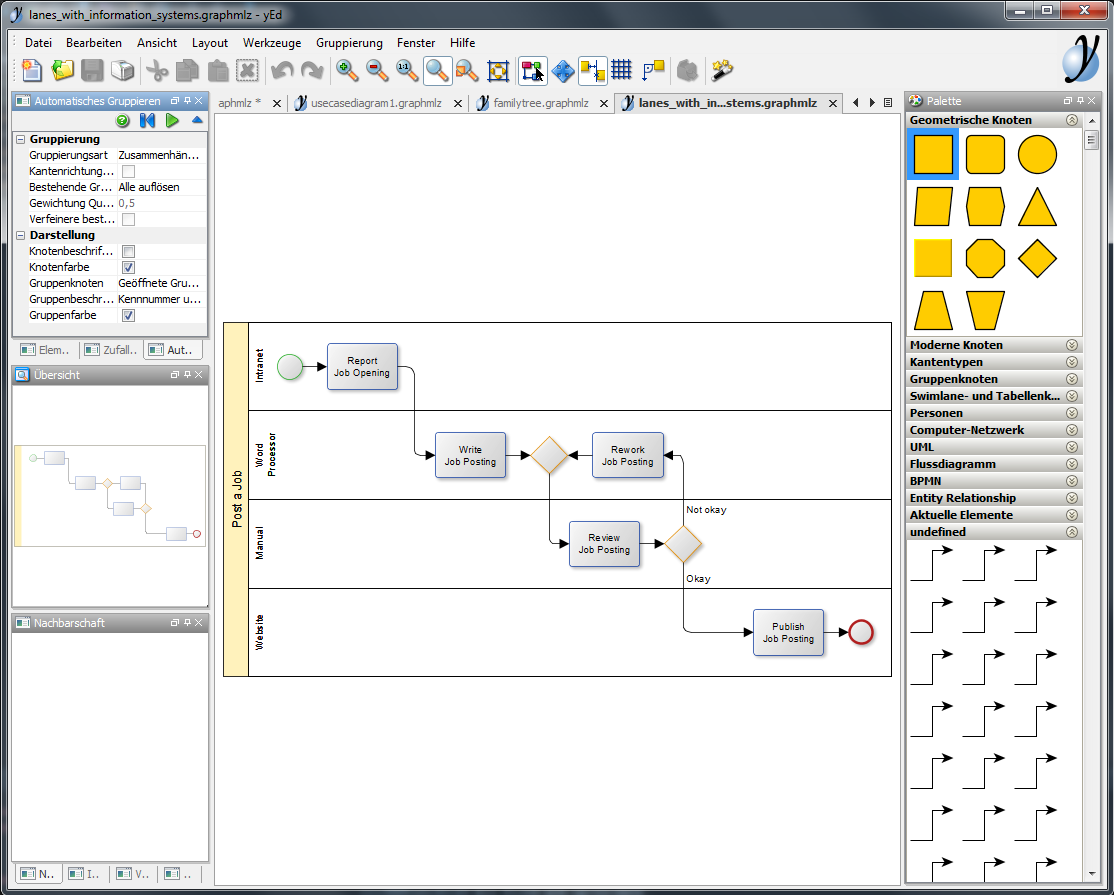
\includegraphics[width=0.85\textwidth]{bilder/screenshot_yed.png}
	\caption{Screenshot yEd während Autotest, man beachte die in Tabs geöffneten, 
	verschiedenen Graphen}
	\label{fig:screenshot_yed}
\end{figure}

\begin{figure}
	\centering
	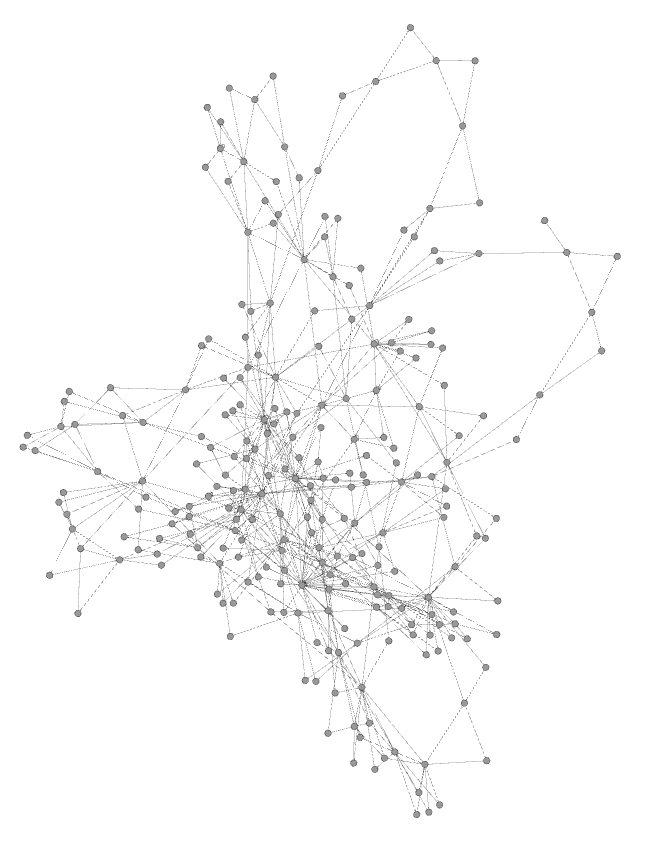
\includegraphics[width=0.85\textwidth]{bilder/model_yed_notext_yh.png}
	\caption{mit Gephi und dem Yifan Hu Algorithmus\cite{hu2005efficient}
    visualierte Graphausgabe des Autotesters über yEd, hoher Zoomfaktor, keine Beschriftungen.}
	\label{fig:screenshot_yed_yh}
\end{figure}

\begin{figure}
	\centering
	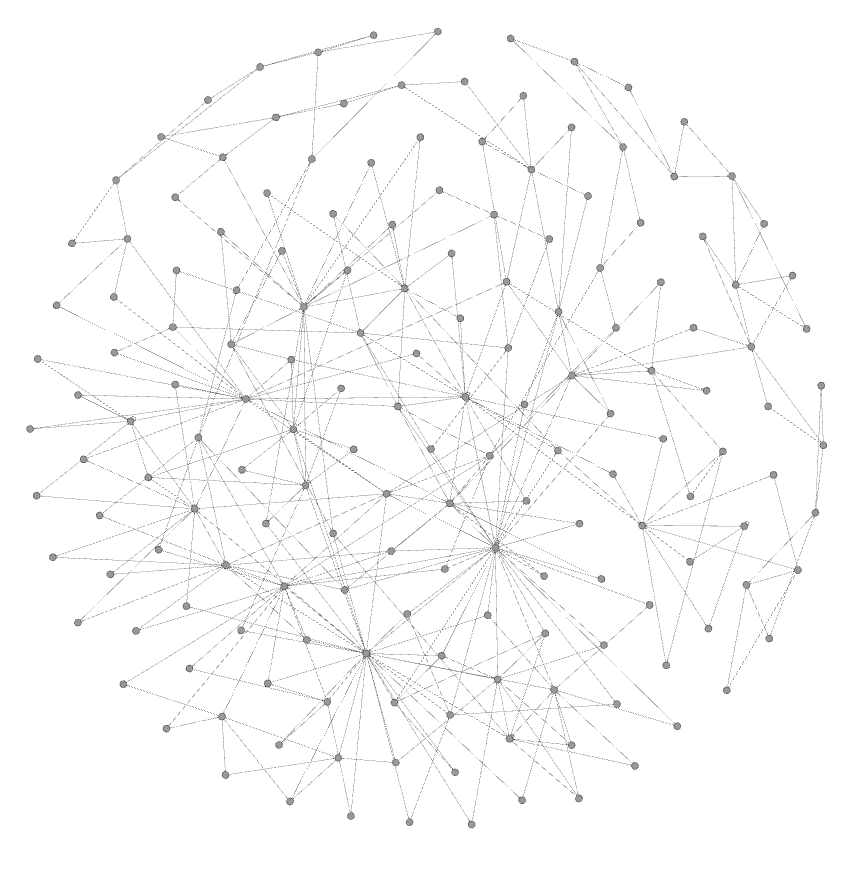
\includegraphics[width=0.85\textwidth]{bilder/model_yed_notext_rf.png}
	\caption{mit Gephi und dem Fruchterman Reingold Algorithmus\cite{SPE:SPE4380211102}
    visualierte Graphausgabe des Autotesters über yEd, hoher Zoomfaktor, keine Beschriftungen.}
	\label{fig:screenshot_yed_rf}
\end{figure}

Als dritte Applikation zum Testen wurde der yEd Graph Editor 
in der aktuellen Version 3.14.4 gewählt,
eine eigenständige Desktopapplikation vergleichbar mit Gephi.
Besonderheiten bezüglich dieses Tests sind z.B., dass yEd Verschleierung
einsetzt, im Englischen Obfuscation genannt. Da die Java-Programmiersprache
Just-In-Time kompiliert wird, enthalten die \glqq{}binären\grqq{}
Dateien noch fast alle Informationen des Quellcodes, und es lässt sich ohne
großen Aufwand äquivalenter Quellcode daraus gewinnen. Dies ist für
Kopierschutz natürlich ein gewaltiges Problem. Im Vergleich dazu lassen
sich auf CPU-Instruktionen kompilierte Programme (sagen wir von C oder C++ aus)
nicht einfach oder eindeutig wieder in Quellcode umwandeln, und der Kompilierer
hat auch die Wahl, sämtliche nutzbaren Meta-Informationen wie Funktionsnamen
zu entfernen.

Eine Lösung dieses Problems für Java ist Obfuscation oder
Verschleierung. Hierbei wird ein Programm zunächst normal kompiliert. 
Danach aber wird vor der Veröffentlichung eine vollautomatische 
Refaktorisierung aller Klassen und Methoden vorgenommen.
Diese hat lediglich zum Ziel, die Bezeichnungen zu ändern. So wird
zum Beispiel aus \glqq{}HauptMenueKlasse\grqq{} schlicht \glqq{}A\grqq{}.
Aus \glqq{}WichtigeFunktion(EingabeKlasse sinnvollerParameterName)\grqq{}
wird \glqq{}a(B a)\grqq{}. Das Resultat ist funktional identisch mit dem
Original, verhält sich also genau gleich, aber eine Begutachtung des
Codes mithilfe eines Dekompilierers ist schwierig bis unmöglich.
Eine kleine Verbesserung der Anwendungsleistung ist ein Nebeneffekt:
Die kürzeren Bezeichnungen sorgen für leicht schnellere Aufrufe, da
kürzere Zeichenketten verglichen werden müssen.

Für den Autotester hat Verschleierung keinerlei Bedeutung, da Aufrufe
an die Swing-API (oder Systemaufrufe oder Aufrufe an nicht verschleierte 
Bibliotheken) nicht versteckt werden können. Oder: So lange ein Programm
lauffähig ist, ist es maschinell auch lesbar. Die zur Identifikation von Komponenten
benutzten Informationen wie Fenstertitel lassen sich ebenfalls nicht verschleiern,
ohne den Nutzen der Anwendung zu zerstören. Was dem Autotester eher
zu schaffen macht, ist die erhebliche Komplexität des Programms und
insbesondere auch die vielen Beispielprojekte, die über Schaltflächen
zugänglich sind. Seiner Natur entsprechend, probiert der Tester diese
natürlich alle aus, was in Änderungen des Hauptfensters resultiert, was
weitere Tests nach sich zieht etc. Betrachtet man die visualisierten
Ausgaben des Zustandsgraphen \ref{fig:screenshot_yed_yh} und 
\ref{fig:screenshot_yed_rf}  auf Seiten \pageref{fig:screenshot_yed_yh} 
und \pageref{fig:screenshot_yed_rf}, sieht man den Unterschied zu vorherigen
Anwendungen sofort. Der Graph erscheint verteilt, ohne klares Zentrum
oder Ursprungspunkt. Dies liegt an den Beispielprojekten, die praktisch
eigene Mini-Ursprungspunkte darstellen. Daraus folgen fast 1700
Eingabeelemente und 74 Fenster, die vom Autotester durchsucht
bzw. ausprobiert werden mussten. Erschwerend kam noch hinzu,
dass eine Sprachumschaltung enthalten ist, welche die Metainformationen
verändert, auf denen die Graphbildung aufbaut. Fenstertitel
unterscheiden sich im deutschen und englischen Modus voneinander.


\subsection{Beispiele für gefundene Probleme yEd}

Nachdem durch iterative Erweiterung der Bannlisten/Blacklists
ein vollständiger Durchlauf des Autotesters über yEd erreicht wurde,
konnte damit begonnen werden, die Logdateien auf Fehler zu
durchsuchen. yEd verfügt über eine integrierte Ausnahmebehandlung,
die jeden Absturz zu verhindern sucht. Anstattdessen öffnet yEd eine
Fehlermeldung, was sehr löblich ist, aber im Vergleich zu FirstSpirit
nicht ideal. Dieses meldet Ausnahmen nur im Hintergrund und leitet
diese automatisch an den Online-Bugtracker von e-Spirit weiter,
sodass die Entwickler sich darum kümmern können und auch gleich
Statistiken darüber bekommen, welche Fehler wie häufig auftraten.
Es gelingt dem Autotester auch hier, unvollständige Fallabdeckung
und sogar zumindest ein kritisches Problem aufzudecken.

Als erstes Beispiel diene der schlichte Fall unerwarteter Zeichenketten:

\begin{lstlisting}[float=!ht,label=fmjson,caption={Ausnahme bei Eingabe einer Nicht-Zahl}]
java.lang.NumberFormatException: For input string: "<a"
at java.lang.NumberFormatException.forInputString[...]
at java.lang.Integer.parseInt(Integer.java:580)
at java.lang.Integer.parseInt(Integer.java:615)
at y.E.R.?(Unknown Source)
at y.E.R.?(Unknown Source)
at y.E.uA$A.setText(Unknown Source)
at espirit.mpoloczek.CrawlerTester$EDTCompliantTextSetter.run[...]
\end{lstlisting}

Die Applikation erzeugt eine unbehandelte Ausnahme, wenn in einem
Textfeld etwas eingegeben wird, das keine Zahl ist. Die korrekte Behandlung
einer solchen Situation wäre das Abschalten des entsprechenden Eingabeelements,
bis eine korrekte Eingabe erfolgt. Dies ist eine der häufigsten Fehlerquellen,
die vom Autotester aufgedeckt werden. Aufgrund der Verschleierung von
yEd ist es nur dem Entwickler selbst (hoffentlich) möglich, zu sagen,
was genau \glqq{}y.E.uA\$A\grqq{} ist und wie dieser Fehler im Quellcode
zu beheben wäre.

Als zweiter Fund dient die Schaltfläche \glqq{}Knotenüberlappungen auflösen\grqq{}.
Zum Zeitpunkt dieser Eingabe war eines der Beispiel-Graph-Projekte geöffnet.
Aus dem folgenden Abschnitt der Logdatei geht hervor, dass nach Betätigung
dieser Schaltfläche mindestens zehn Sekunden lang gar nichts mehr geschah,
der Autotester also darauf wartete, den Kontrollfluss von der Implementation der
Schaltfläche wieder zurückzuerhalten, während yEd irgendetwas tat. Der
folgende Fehler \glqq{}OutOfMemoryError: Java heap space\grqq{}
deutet auf einen Programmierfehler in yEd hin, der zu einer Endlossschleife
bis hin zum Absturz der Java Virtual Machine führt. Die Applikation \glqq{}hängt\grqq{}, bis
dieser Absturz erfolgt. Leider verfügt die Logdatei des Autotesters nicht über einen
detaillierten Kontext (woher auch), aber dies stellt einen schweren Fehler in yEd
dar und sollte baldmöglichst behoben werden.

\begin{lstlisting}[float=!ht,label=fmjson,caption={Ausnahme yEd durch Schaltfläche \glqq{}Knotenüberlappungen auflösen\grqq{}}]
espirit.mpoloczek.CrawlerTester pseudoClickButton
about to pseudo click component JMenuItem: [Knotenueberlappungen ...]
espirit.mpoloczek.CrawlerTester$TimerRunner run
No actions were taken for 10 seconds, deadlock situation??
---> BEGIN ERROR
java.lang.OutOfMemoryError: Java heap space
at com.sun.java.help.search.Query.makePenaltiesTable[...]
at com.sun.java.help.search.Query.<init>(Query.java:43)
at com.sun.java.help.search.Search.<init>(Search.java:51)
at com.sun.java.help.search.QueryEngine.processQuery[...]
at com.sun.java.help.search.DefaultSearchQuery.run[...]
at java.lang.Thread.run(Thread.java:745)
---> END ERROR
\end{lstlisting}



\section{Vergleich mit klassischen Tests}\label{section:testcomparisonclassic}

Ein Vergleich mit halbautomatischen Methoden oder gewöhnlichen Unit-Tests
ist erst einmal schwierig, da diese auf anderen Prinzipien aufbauen.
Üblicherweise ist das Ziel die Überprüfung der Korrektheit des Programms.
Um eine Aussage über Korrektheit treffen zu können, sind kontextuelle
Informationen über ein Programm bzw. das gewünschte Verhalten notwendig.
Einem vollautomatischen Ansatz stehen diese Informationen schlicht nicht
zur Verfügung. Das hier vorgestellte Konzept ist auch nicht als Ersatz 
klassischer Tests gedacht oder in irgendeiner Form äquivalent.

Getreu dem Zitat von Dijkstra \footnote{ACM Turing Lecture 1972},
nach dem die Abwesenheit von Fehlern nicht bewiesen werden kann,
zielt der Autotester in eine andere Richtung. Es wird versucht, so viele
unerwartete Situationen und resultierende Fehler zu erzeugen, wie
irgendwie möglich. Man kann ihn also als ein Komplement bzw. eine Addition
zu klassischen Tests verstehen bzw. Einsetzen.

Ein Durchlauf des Autotesters ist verglichen mit Unit Tests und den
meisten Regressionstests sehr langsam. Ein vollständiger Durchlauf
über FirstSpirit dauert ungefähr 20 Minuten. Leider gibt es für die
Emulation menschlicher Eingaben und der Wartezeit für die Verarbeitung
dieser Eingaben durch das Programm keine guten Alternativen.
Man bedenke allerdings: Derselbe Test durch einen Menschen würde
noch erheblich länger dauern und die üblichen menschlichen Fehlerquellen
beinhalten, die das Ergebnis zusätzlich beeinflussen. Auch handelt es
sich bei der Entwicklerversion von FirstSpirit um ein massives
Konstrukt mit Serverbedingt behäbigen Reaktionszeiten und gewaltigem
Funktionsumfang, also vielen (beinahe eintausend) zu testenden Elementen.

%%% TeX-master: "../main.tex"
% kapitelfazit.tex
\chapter{Fazit und Ausblick}\label{chapter:expansion}

Im Laufe dieser Arbeit wurde ein neuartiges Konzept zum vollautomatischen
Test graphischer Oberflächen vorgestellt, eine Implementation wurde
vorgestellt, und konkrete Tests durch den nach dem Konzeptprinzip
funktionierenden Tester demonstriert. In diesem Kapitel werden
die gewonnenen Erkenntnisse und Ergebnisse noch einmal zusammengefasst 
und Ansätze für eine weitere Entwicklung des Konzept werden aufgezeigt.


\section{Konzeptumsetzung}\label{section:conceptimplement}

Es ist gelungen, eine nahezu vollständige Automation des destruktiven
Testprozesses umzusetzen. Mit nur einigen wenigen unbedingt nötigen Angaben
zur zu testenden Oberfläche erledigt der Autotester völlig selbsttätig
alle weiteren Schritte, die viele klassische bzw. gewöhnliche Tests aufwändig
in der Implementation oder auch der Wartung machen. Es ist nicht notwendig,
dem Tester eine Liste der zu prüfenden Elemente vorzugeben. Er nutzt
Eigenschaften der Java-Swing-API aus, um selbst alle zu Eingabeverarbeitung
fähigen Komponenten einer graphischen Oberfläche zu finden. Alle diese
Elemente werden dann systematisch geprüft. Um möglichst viele
mögliche Fehlerzustände zu finden, wird diese Reihenfolge von Durchlauf
zu Durchlauf zufällig variiert.

Zeichenketten akzeptierende Eingabekomponenten werden mit einer
Vielzahl bekanntermaßen problemträchtiger Strings bombardiert,
die übliche übersehene Validationen oder Verifikationen von
Eingaben aufdecken. Sich öffnende Zusatzelemente der Oberfläche
oder auch komplett neue Fenster werden automatisch erkannt, mit
der Eingabe, die vermutlich zu ihrem Erscheinen geführt hat, verknüpft,
und ebenfalls systematisch auf Komponenten durchsucht und getestet.

Es bestehen sowohl Möglichkeiten der manuellen Vorgabe von
Ausnahmen im Testablauf als auch vollautomatische Routinen,
die vorzeitige Beendigung des Tests verhindern und die
Effizienz des Testablaufs erhöhen. Nach nur einigen wenigen iterativen
Durchläufen mit menschlicher Beobachtung sollte es möglich sein, 
jede beliebige Java-Swing-Applikation mit dem Autotester vollständig 
prüfen zu lassen. Bei einem vorzeitigen Beenden muss lediglich die
Logdatei auf die zuletzt getätigten Eingaben geprüft werden,
um dann eine simple Ausnahmeregel in die Konfigurationsdatei zu schreiben.

Nach jedem erfolgreichem Durchlauf erstellt der Tester
eine Textdatei im graphML-Format, welche mit den meisten
verfügbaren Applikationen zur Graphvisualisierung in ein
ansprechendes Format gebracht werden kann. So ist es möglich,
ein Abbild der getesteten Oberfläche und aller ihrer Zustände 
zu schaffen, welches gewissermaßen von einem blinden Maler stammt.
Bei Betrachtung dieses Graphen kann ein Mensch häufig
ohne jegliche Kenntnis des Programms Annahmen über seinen Zweck
und den Bedienungsablauf treffen.

Der Autotester schafft es regelmäßig, ohne irgendeine Kenntnis des zu
testenden Programms oder seiner Funktion alle Möglichkeiten
der Eingabe auszuprobieren, und dabei manchmal Fehler durch unerwartete
Eingaben im getesteten Programm auszulösen.
Indem diese gefundenen Fehler dann behoben werden, erhöht sich die
Softwarequalität des getesteten Programms. Das Ziel des Konzepts
war es nicht, Korrektheit zu beweisen oder zu testen. Dafür
sind kontextuelle Informationen notwenig, die bis zur Existenz
künstlicher Intelligenz schlicht von Menschen vorgegeben werden müssen.


\subsection{mögliche Erweiterungen}

Die größte Einschränkung, wenn man sie denn als solche bezeichnen
kann, ist die auf Java-Anwendungen, die die Swing-API verwenden.
Ein Java-Entwickler ist natürlich nicht gezwungen, diese zu verwenden,
und es gibt beispielsweise mit SWT
\footnote{ \url{ https://www.eclipse.org/swt/ }} zumindest eine 
verbreitete Alternative. Auch ist die Swing-API auf Android
nicht oder nur in abgewandelter Form vertreten. Man könnte
den Tester also dahingehend erweitern bzw. neu implementieren,
dass auch Java-SWT oder Android-View
\footnote{ \url{ https://developer.android.com/reference/android/view/package-summary.html }} 
automatisch getestet werden könnten. Für Android müsste aber
vermutlich das gesamte Verhalten des Testers geändert werden,
um den Eigenschaften des Android-Betriebssystems entgegenzukommen,
und Unterstützung für den Android-Emulator
\footnote{ \url{ https://developer.android.com/tools/help/emulator.html }} 
sowie die Debug-Verbindung adb
\footnote{ \url{ https://developer.android.com/tools/help/adb.html }} 
bieten sich ebenfalls als nützlich und naheliegend an.
Im Fall von SWT müssten lediglich die spezifischen Schnittstellen
des SWT (verglichen mit Swing) analog behandelt werden, und 
das Ereignis eines sich öffnenden Fensters ist vermutlich auch
anders implementiert. Aber im Gegensatz zu Android verhält
sich eine SWT-Applikation identisch zu einer Swing-Applikation,
weshalb der Tester selbst unverändert übernommen werden könnte.

Möchte man größere Ziele erreichen, sind auch weitreichende
Erweiterungen vorstellbar. So könnte man Computersehen bzw.
Computer Vision verwenden, um auf einem beliebigen Bildschirm
alle Schaltflächen und Eingabefelder zu erkennen. Diese sind
für den Menschen recht einfach zu erkennen, für einen
Computer wäre dies schon eher eine Herausforderung. Aus den
Kontrasten eines Bildes würde dieser auf Formen schließen
und so versuchen, die üblichen Rechtecke und seltener Kreise
zu erkennen, die Schaltflächen signalisieren. Dann müsste
tatsächlich der Mauszeiger zu diesen Koordinaten bewegt
und betätigt werden (dies könnte durch Nebeneffekte seitens
der Anwendung verhindert werden). Ebenso müsste der Computer
versuchen, aus der Änderung eines Großteils des Bildes
in Quadratischer Form auf das Auftreten eines Popups zu 
schließen und entsprechend zu reagieren, und dies möglichst,
ohne ein Popup mit der Anzeige eines gewünschten Bildes
oder einer sonstigen Information innerhalb desselben
Fensters zu verwechseln.


% Anhang
\appendix

%Abbildungsverzeichnis
\listoffigures
\addcontentsline{toc}{chapter}{Abbildungsverzeichnis}
\cleardoublepage

% Algorithmenverzeichnis
\listofalgorithms
\addcontentsline{toc}{chapter}{Algorithmenverzeichnis}
\cleardoublepage

% Literaturverzeichnis
\bibliographystyle{gerplain}
\bibliography{literatur/literatur}
\addcontentsline{toc}{chapter}{\bibname}

% Erklaerung
\thispagestyle{myheadings}
\markboth{}{ERKLÄRUNG}
\addcontentsline{toc}{chapter}{Erklärung}
% erklaerung.tex
\cleardoublepage
\normalsize
Hiermit versichere Ich, dass ich die vorliegende Arbeit selbstständig verfasst habe und keine anderen als die angegebenen Quellen und Hilfsmittel verwendet sowie Zitate kenntlich gemacht habe.\\\\
Dortmund, den \today \\\\\\\\
Matthäus Poloczek
% EOF
\cleardoublepage

\end{document}
% EOF
